\chapter{Información Biológica}
\label{cap:informacion}

Habiendo explicado los diferentes métodos de ajuste en el capítulo \ref{cap:microscopia} y aclarado como obtener la proporción de caspasa activa a partir del estado del ensamble de fluoróforos en el capítulo \ref{cap:modelo}, procedemos a presentar el experimento realizado del cual se obtuvieron los datos para analizar. Dicho experimento se realizó en el instituto Max Planck de alemania en el marco del proyecto \ening{Biocompatible multitasking nanoparticles for spatiotemporally resolved monitoring and photoinactivation of cancer cells and antibiotic resistant bacteria} financiado por el \ening{Deutsche Forschungsgemeinschaft} (DFG).

En este capítulo, los métodos desarrollados y explicados previamente serán aplicados al sistema en estudio para obtener información valiosa sobre el funcionamiento de este, además de brindar una mayor comprensión sobre los métodos utilizados. Por otro lado, se analizarán las posibles fuentes de error y falencias experimentales, así como posibles correcciones al protocolo experimental.


%%%%%%%%%%%%%%%%%%%%%
\section{Armado Experimental}

Si bien el experimento no se realizó en el laboratorio, este consistió fundamentalmente en preparar un cultivo celular que exprese los biosensores para las caspasas deseadas, para luego proceder a estimular la inicialización de apoptosis en estas células y observar la dinámica de los biosensores. El primer paso fue desarrollar mediante ingeniería genética el plásmido que sería transfectado a la célula. Éste consiste en una secuencia de ADN que contiene la información necesaria para que la célula en cuestión pueda sintetizar alguna proteína en particular. Durante la transfección, se condiciona a la célula para que pueda recibir material genético externo, por medio del plásmido, para luego poder procesarlo como propio.

Una vez que las células expresan los biosensores transfectados, estas deben ser inducidas para entrar en apoptosis mediante algún estímulo como staurosporina o TNF-$\alpha$, si se desea inicializar por la vía extrínseca, o especies reactivas del oxígeno, si se desea estimular la vía intrínseca. Habiendo inducido a la célula, solo resta adquirir imágenes de los observables fotofísicos para proceder a su análisis y estudio del sistema biológico.

\subsection{Diseño de Biosensores}

Tres biosensores basados en homoFRET fueron diseñados para luego ser transfectados a las células en estudio. Las combinaciones de fluoróforos utilizados fueron TagBFP con mCerulean, mCitrine con mCitrine y mCherry con mKate, cuyos espectros se muestran en la figura \ref{fig:EspectroFluos}. Los biosensores se construyeron insertando el segundo fluoróforo amplificado por PCR y delimitado por los sitios de restricción de Spe1 y Sal1 y conteniendo un codon STOP en los sitios de restricción Spe1/Sal1 de un vector-C1 (Clontech). Adicionalmente, el producto de PCR tenía una secuencia de unión en el extremo 5'. Estos plásmidos se utilizaron como controles no clivables. Por otro lado, para construir los sensores clivables por la caspasa, se utilizaron las secuencias que codificaban para los sitios de clivado de las caspasas-3, -8 y -9 (DEVD, IETD-IETD, LEHD, respectivamente) fueron amplificadas por PCR y delimitadas por sitios de restricción BSP1 y Spe1, y luego subclonados a los sitios de restricción correspondientes en los plásmidos de control no clivables, volviendolos plásmidos que codifican para el sensor clivable.

\begin{figure}
    \centering
    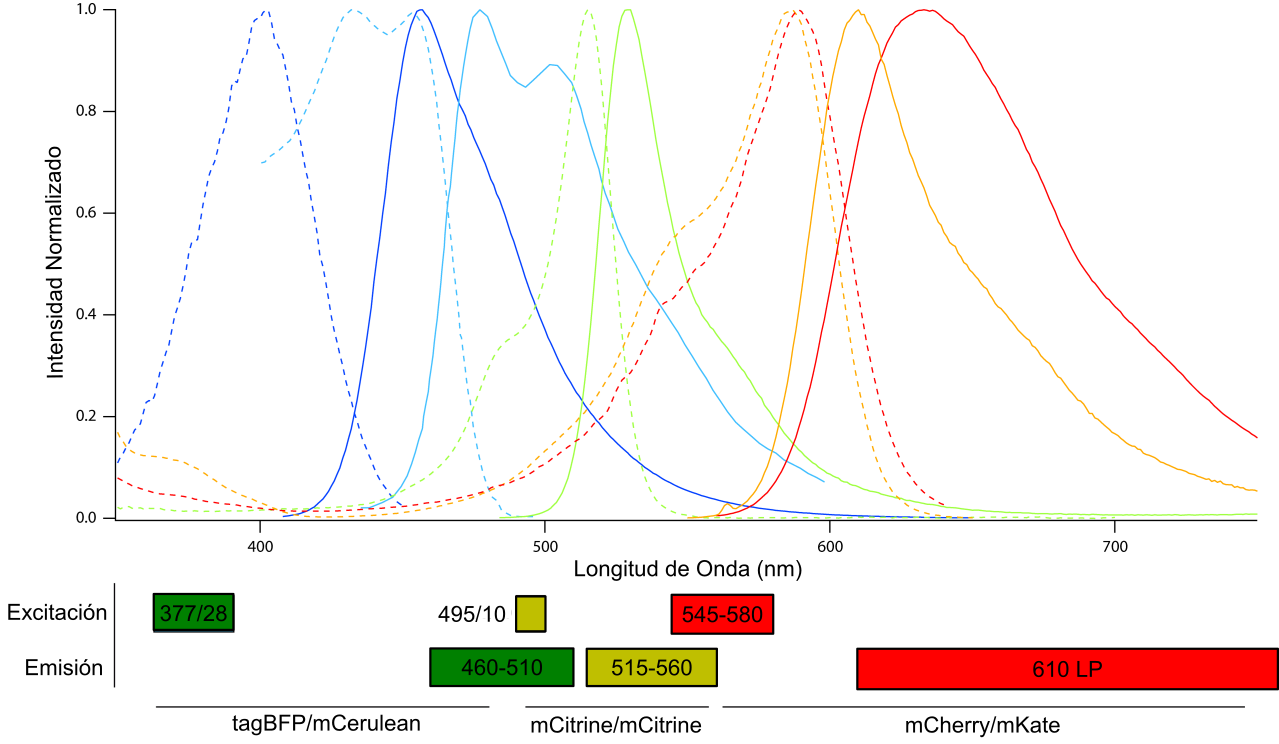
\includegraphics[width=0.9\textwidth]{./img/Cap4/spectra_w_filters.png}
    \caption{Espectro de excitación y emisión de los fluoróforos utilizados. Se muestra también los filtros utilizados en la adquisición.}
    \label{fig:EspectroFluos}
\end{figure}

\subsection{Cultivo Celular}

Se cultivaron células Hela en medio DMEM (PAN Biotech) suplementado con 10$\%$ suero fetal de cabra (FCS, Gibco), 100 U/ml de penicilina, 100$\mu$g/ml de streptomicina, 1$\%$ de L-glutamina y 1$\%$ de aminoácidos no esenciales (todos de PAN Biotech) a 37$^{\circ}$C y 5$\%$ de CO$_2$ en una incubadora humidificada. El día anterior a la transfección las células fueron traspasadas a discos de 8 \ening{wells} (LabTekII, Nalgene) a una densidad de $3\times10^4$ células. La transfección se concretizó utilizando Fugene 6 (Promega) siguiendo el protocolo del manufacturante. 20 horas después de la transfección, las células fueron observadas en DMEM sin rojo fenol (PAN Biotech) y 0$\%$ FCS en presencia de 1$\mu$M de staurosporina (Sigma Aldrich, Alemania) junto con 10$\mu$g/ml de ciclohexamida (Sigma Aldrich, Alemania) para inducir apoptosis e inhibir la síntesis proteíca.

\subsection{Adquisición de Imágenes}

Las imágenes fueron adquiridas mediante un setup customizado en Alemania. Se utilizó un microscopio invertido Olympus IX-81 equipado con un sistema de iluminación MT20. Se adicionaron tres polarizadores dicroicos Meadowlark Optics, Frederick, Colorado, US), uno en el camino óptico de excitación del microscopio y los otros dos fueron colocados con sus ejes perpendiculares entre sí en una rueda de filtros en el exterior del microscopio (ver figura \ref{fig:armadoExp}). La fluorescencia se colectó utilizando un objetivo de aire de 20$\times$ y apertura numérica de 0,7. Las imágenes en las polarizaciones paralela y perpendicular se adquirieron secuencialmente utilizando una cámara CCD Orca (Hamamatsu Photonics, Japan). El software CellR (Olympus, Alemania) fue utilizado para controlar la adquisición. Previo a cada experimento se tomaron imágenes de una muestra de referencia, siendo esta fluoresceína diluida. Estas se tomaron a 37$^{\circ}$C usando un sistema de control de temperatura que consistió en un calentador de objetivo y el calentador de especimen Stable Z (Bioptechs Inc., Butler, PA, USA). Estas últimas se utilizaron para calibrar el sistema calculando el factor G.

\begin{figure}
    \centering
    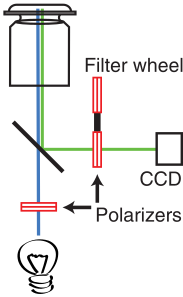
\includegraphics[width=0.2\textwidth]{./img/Cap4/ArmadoExp.png}
    \caption{Esquema del camino óptico del armado experimental donde se detalla la ubicación de los polarizadores utilizados.}
    \label{fig:armadoExp}
\end{figure}

\subsection{Procesamiento de Imágenes}

En primer lugar, se utilizaron las imágenes adquiridas de la solución diluida de fluoresceína para corregir inhomogeneidades en la iluminación. Para ello, se dividio pixel a pixel, las imágenes de ambas polarizaciones con su correspondiente imagen de fluoresceína.Dado que el valor de anisotropía de la fluoresceína es muy cercano a cero, este procedimiento también sirve para corregir con el factor G, como se explicó previamente, el factor G da cuenta de las diferencias en sensibilidad de cada dirección de polarización observada.

A continuación, se sustrajo el ruido de fondo de las imágenes usando como valor de ruido de fondo la intensidad promedio de una región afuera de las células. Luego, debido a que los polarizadores introducen un corrimiento entre las imágenes de ambas polarizaciones, y considerando que este es el mismo para todas las imágenes, se busco corregir este corrimiento.

Una vez corregidas las imágenes adquiridas, se procedió a generar máscaras mediante un software de análisis de imágenes llamado \ening{Cell Profiler}. Este permitió identificar a las células como objetos, además de delimitar sus bordes. Para ello, el software selecciona un umbral de intensidad a partir del cual considera como parte del objeto todos los pixeles que sean más brillantes que el umbral, además de considerar regiones separadas como objetos distintos. Luego, se calculó el promedio de las intensidades paralela y perpendicular de cada célula, para calcular después la anisotropía utilizando la ecuación \ref{eq:anisotropia}. Un esquema de este procedimiento se presenta en la imágen \ref{fig:esqexp}.

\begin{figure}
    \centering
    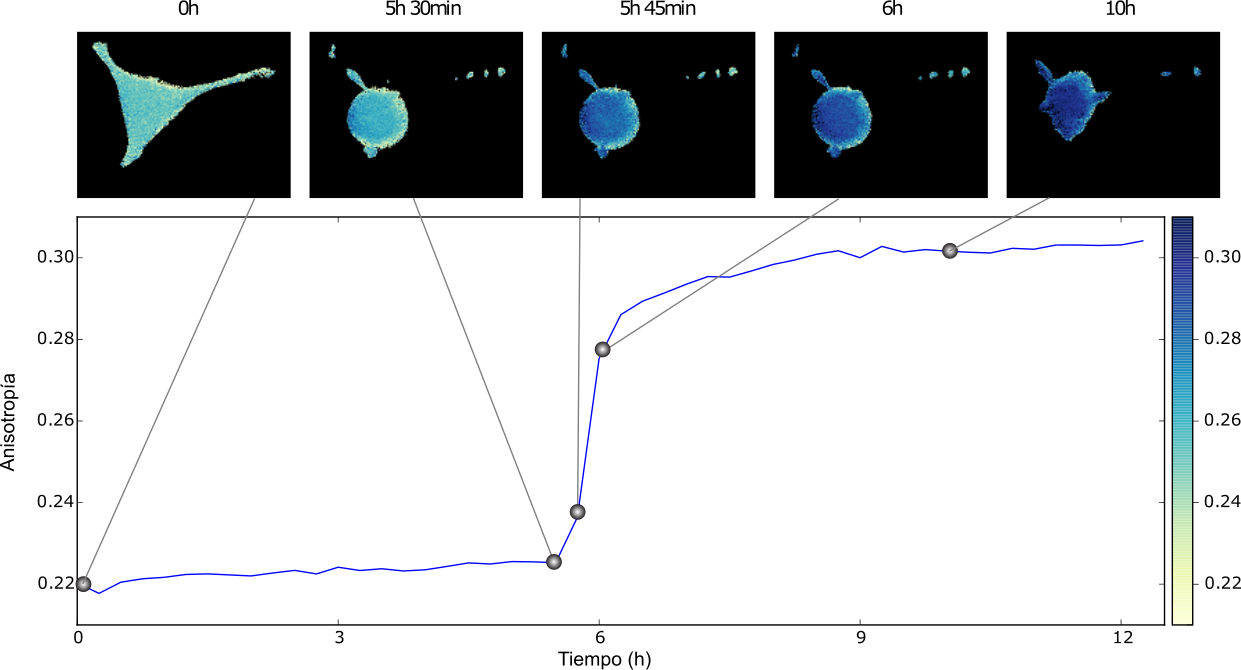
\includegraphics[width=0.9\textwidth]{./img/Cap4/EsqExp.png}
    \caption{En la sección superior se presenta una serie temporal de las imágenes adquiridas de una célula en particular durante el proceso de apoptosis. Se presenta en escala de azules la anisotropía observada en cada pixel. Puede apreciarse como cambia la máscara de la célula a medida que disminuye la intensidad de algunos pixeles. Simultáneamente, podemos apreciar la curva de anisotropía calculada para esta célula.}
    \label{fig:esqexp}
\end{figure}


%%%%%%%%%%%%%%%%%%
\section{Curvas}

Con el objetivo de obtener las curvas de anisotropía e intensidades total, paralela y perpendicular, que serían utilizadas para evaluar el sistema se realizaron los siguientes procedimientos. En primer lugar, luego de recibir los datos, se ajustaron todas las curvas de anisotropía por una función sigmoidea, es decir,

\begin{equation}
    f(x) = base + \frac{amplitud}{1+e^{k(x-x_0)}},
\end{equation}

\noindent donde la base y amplitud se refieren a los valores estables que adquiere la función para x mucho menores o mayores que $x_0$, respectivamente. El parámetro $k$ esta asociado con la velocidad de transición de un valor estable al otro, mientras que $x_0$ determina el valor de $x$ para el que la función se halla en el punto medio entre ambos valores. Esta función es la misma que se utilizó en el capítulo \ref{cap:microscopia} para generar la curva simulada de proporción de fluoróforo en estado monomérico.

Dado que la adquisición y el procesamiento de imágenes fue automatizado, muchas de las curvas obtenidas correspondían a artefactos de medición. Con el objetivo de filtrar los más de 3000 objetos identificados, se utilizaron los parámetros de la función sigmoidea para filtrar las curvas correspondientes a células en apoptosis de las que no. De esta forma, se identificaron 121 células con sus 3 curvas correspondientes a los tres biosensores que podían ser analizadas. En la figura \ref{fig:Aniso_ej} se presenta un ejemplo de las tres curvas de anisotropía de cada sensor correspondientes a una misma célula. Por otro lado, en la figura \ref{fig:todas} se muestra una superposición de todas las curvas de anisotropía filtradas y centradas para apreciar su forma funcional.

\begin{figure}
    \centering
    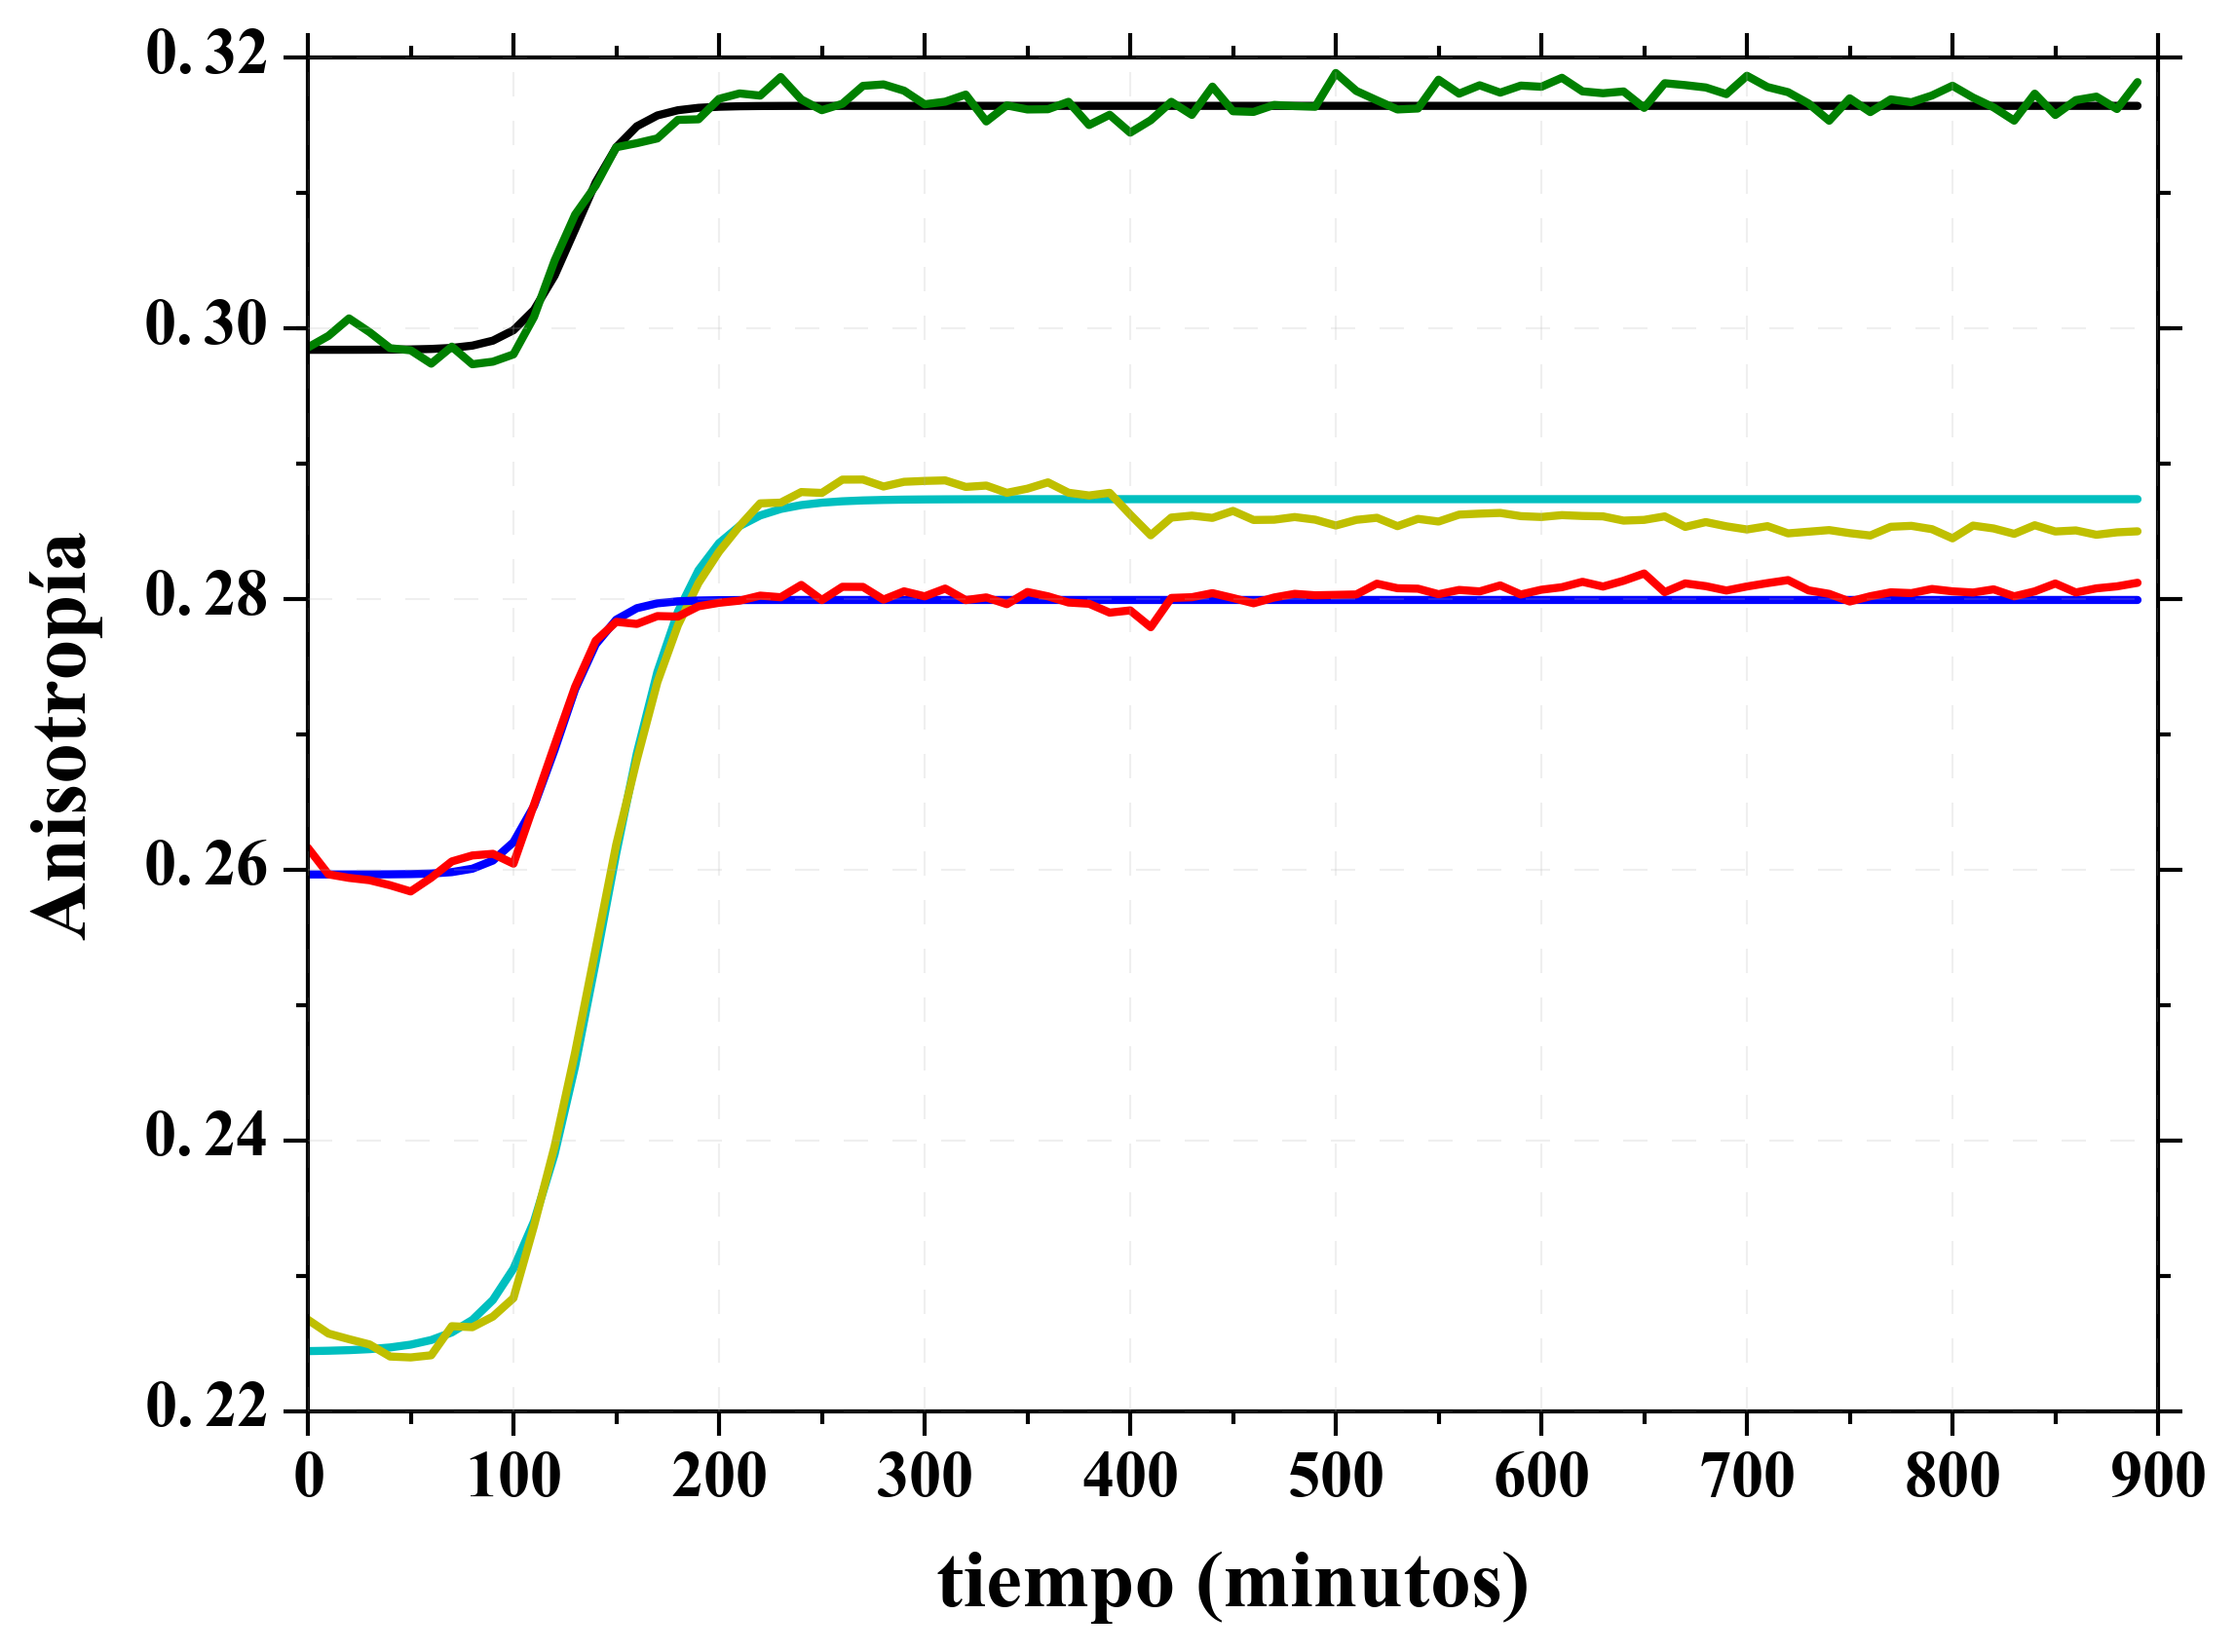
\includegraphics[width=0.6\textwidth]{./img/Cap4/Anisotropia2145.png}
    \caption{Gráfico de anisotropía en función del tiempo de cada sensor correspondientes a una misma célula.}
    \label{fig:Aniso_ej}
\end{figure}

\begin{figure}
    \centering
    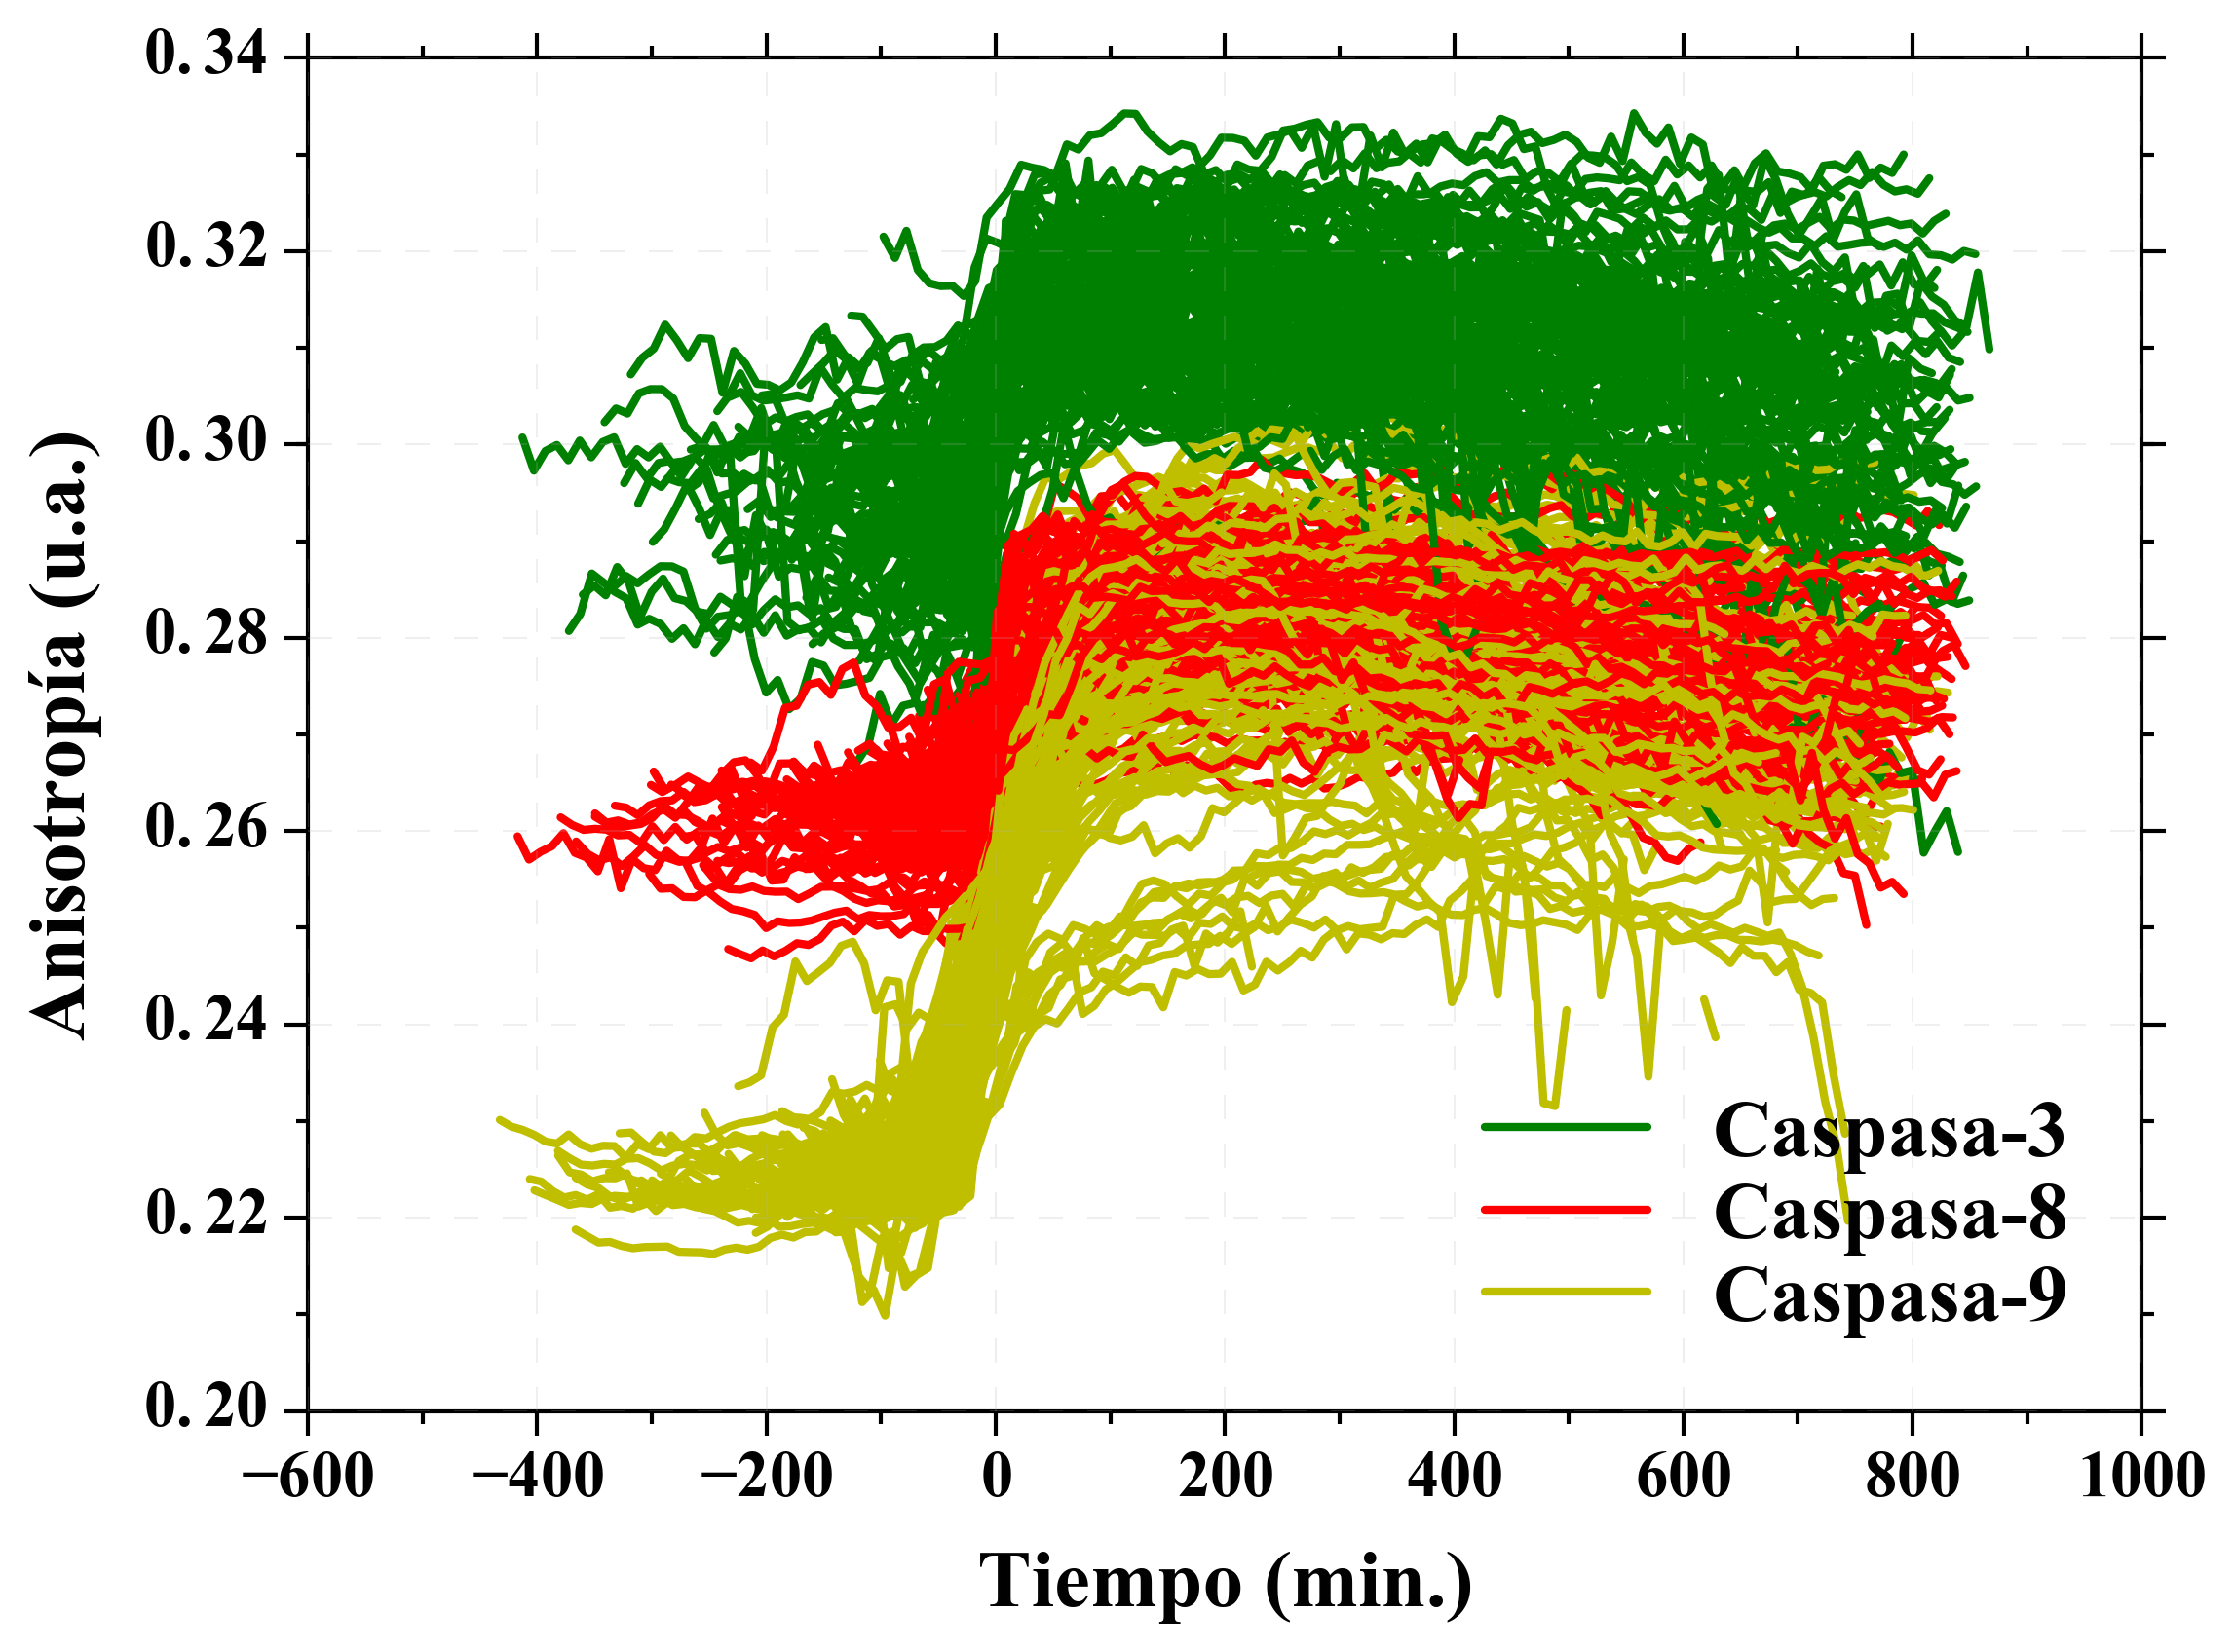
\includegraphics[width=0.6\textwidth]{./img/Cap4/AnisoJuntas.png}
    \caption{Gráfico de anisotropía en función del tiempo de todos los biosensores en todas las células. Se aplicó un corrimiento a todas las curvas para centrarlas y apreciar la forma de estas.}
    \label{fig:todas}
\end{figure}

Considerando que durante la adquisición de imágenes el foco no podía ser controlado automáticamente y teniendo en cuenta que la degradación de proteínas pueden llegar a tener un efecto sobre la anisotropía, se confeccionaron funciones que, basadas en los parámetros obtenidos de los ajustes previos, toman para analizar únicamente la región de la transición. Estas funciones se utilizaron para recortar las regiones de interés en las curvas de anisotropía.

Una vez halladas las curvas que se estudiarán resulta valioso comenzar con un análisis estadístico de los parámetros más importantes disponibles. Entre ellos, podemos estudiar las anisotropías del monómero y dímero, al igual que su diferencia o rango dinámico. Utilizando como hipótesis que el experimento se inicia con la totalidad del biosensor sin clivar y culmina con la totalidad del sensor clivado, se tomaron los diez valores de anisotropía que delimitaban las curvas recortadas para estimar los valores de anisotropía del dímero y del monómero.

\begin{figure}
    \centering
    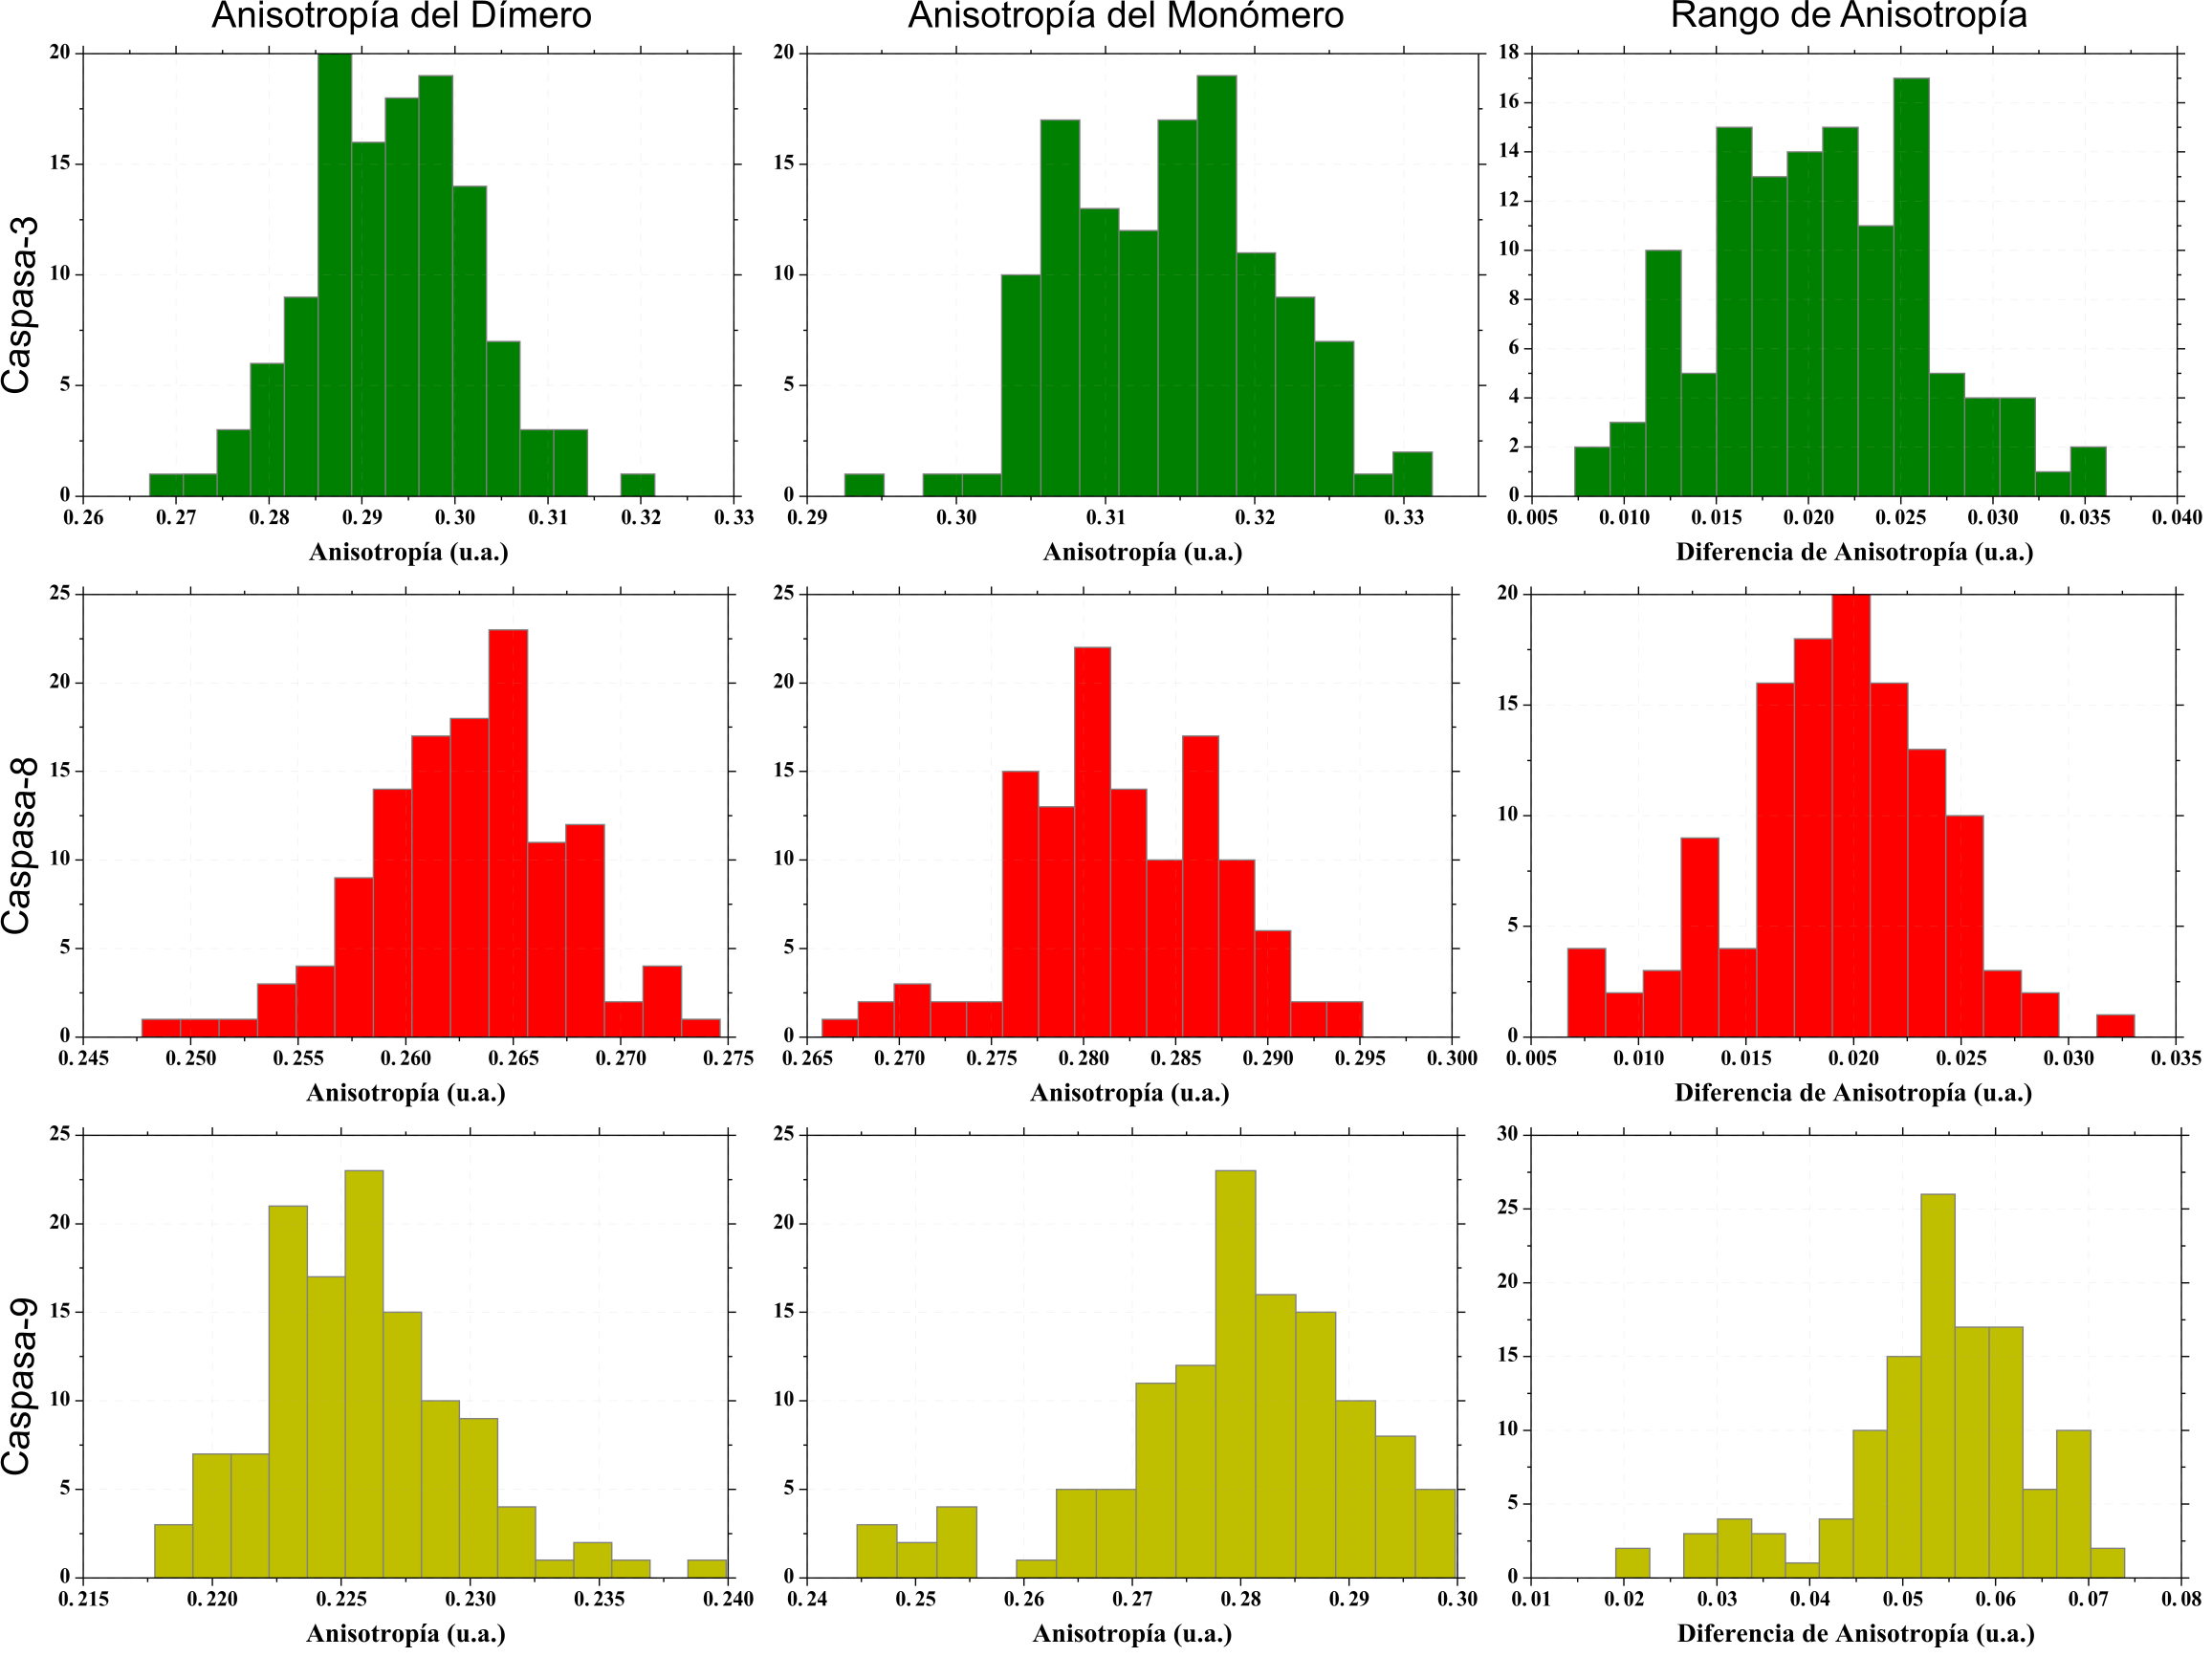
\includegraphics[width=0.9\textwidth]{./img/Cap4/HistogramasAnisos.png}
    \caption{Histogramas de los valores de anisotropía del dímero, anisotropía del monómero y rango de anisotropía hallados para cada par de fluoróforos.}
    \label{fig:HistogramasAnisos}
\end{figure}

En la figura \ref{fig:HistogramasAnisos} se presentan los histogramas de las distintas anisotropías máximas y mínimas obtenidas para cada fluoróforo así como también la diferencia entre ambas para conocer su rango dinámico. En particular, se obtuvieron para tagBFP/mCerulean la anisotropía del monómero fue de 0.3140$\pm$0.0070, la del dímero 0.2933$\pm$0.0088, y la diferencia entre anisotropías fue de 0.0206$\pm$0.0059. Para mCherry/mKate la anisotropía del monómero fue de 0.2819$\pm$0.0055, la del dímero 0.2628$\pm$0.0045, y la diferencia entre anisotropías fue de 0.0191$\pm$0.0048. Por último, para mCitrine/mCitrine la anisotropía del monómero fue de 0.279$\pm$0.012, la del dímero 0.2257$\pm$0.0037, y la diferencia entre anisotropías fue de 0.054$\pm$0.011. 

Por otro lado, si observamos las anisotropías teóricas para los distintos pares de fluoróforos apreciamos que para los dímeros las anisotropías son 0,266 para tagBFP/mCerulean, 0,271 para mCherry/mKate y 0,221 para mCitrine. En estos casos solo la anisotropía del dímero mCitrine/mCitrine se adecua al valor teórico. Si descartamos la hipótesis que comenzamos con la totalidad del sensor en estado dimérico, esperaríamos comenzar con una anisotropía mayor al valor teórico presentado, hecho que solo se cumple para tagBFP/mCerulean y no para mCherry/mKate.

Análogamente, podemos pensar que la totalidad del biosensor es clivado y obtendríamos valores de anisotropía entre los valores individuales teóricos de cada fluoróforo. A saber, para tagBFP 0,346 y para mCerulean 0,32; para mCherry 0,298 y 0,276 para mKate; y mCitrine debería tener un valor de 0,303. En este caso se puede explicar la diferencia entre los valores teóricos y experimentales de la anisotropía del monómero de tagBFP/mCerulean y mCitrine como que no todo el sensor es clivado. En cuanto a mCherry/mKate, las anistropías del monómero se corresponden entre sí.

Debido a que los errores en las anisotropías halladas eran sistemáticos, se estudiaron las posibles fuentes de error. Entre ellas, se pensó que el factor G podía estar mal calculado o incluso podía existir una mala estimación del ruido de fondo que generaría que haya un valor constante sumado en todas las curvas de intensidad utilizadas. Al analizar los valores que debían tener estos errores para recuperar los valores esperados de anisotropía, apreciamos que el error debía ser del orden o mayor que la intensidad observada, por lo que se descarto esta teoría. Con el fin de corregir este problema se planteó que en próximos experimentos se debían agregar casos control para hallar estos valores experimentalmente. Estos casos control consisten en \ening{wells} con biosensores que se encuentran en su totalidad clivados o sin clivar, para obtener una medición de los valores extremos en que se encuentra la anisotropía de cada par de fluoróforos.

%todo{se pueden hacer los mismos estudios para b}

%mCit-mCit: 0.221 --> 0.303 (mCit)
%mKate-mKate: 0.271 --> 0.298 (Cherry) / 0.276 (mKate)
%BFP - Cerulean: 0.266 --> 0.346 (BFP) / NA (Cerulean)


%%%%%%%%%%%%%%%%%%
\section{Estimación de Proporción de Fluoróforo en Estado Monomérico}

Se utilizaron los hallazgos del capítulo \ref{cap:microscopia} para ajustar las curvas experimentales de anisotropía halladas. Se presenta en la figura \ref{fig:Bad_Fits} un par de curvas de anisotropía e intensidad total correspondientes al mismo sensor en la misma célula y ajustadas como se describió previamente. Puede apreciarse la elevada similitud entre las curvas ajustadas y las experimentales, sin embargo, si observamos la curva de anisotropía obtenida a partir de los parámetros obtenidos y la comparamos con la anisotropía experimental, apreciamos que hay grandes diferencias. Se observa el mismo problema para los ajustes de intensidades cruzadas presentados en la misma figura.

\begin{figure}
    \centering
    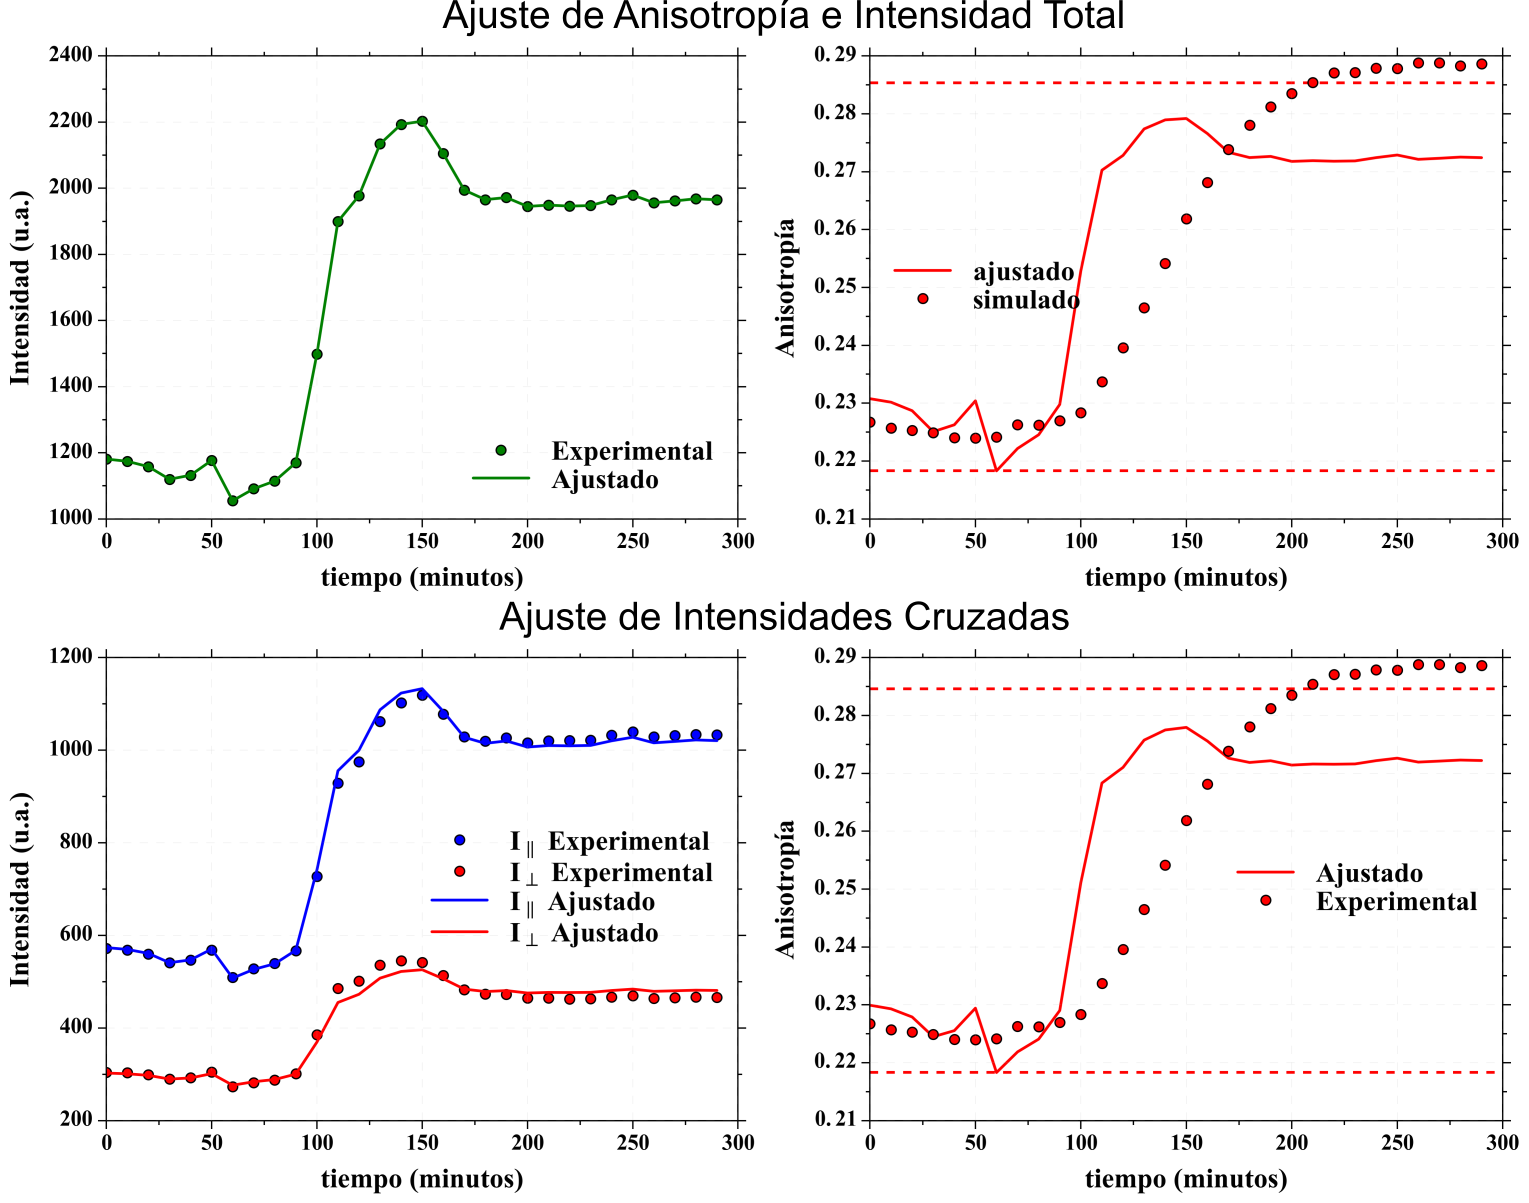
\includegraphics[width=0.9\textwidth]{./img/Cap4/Bad_Fits.png}
    \caption{Ajustes realizados sobre las curvas de anisotropía e intensidad total y sobre las intensidades cruzadas. Puede apreciarse que hay una elevada similitud entre las curvas ajustadas y las intensidades, pero cuando se analiza la anisotropía obtenida a partir del ajuste, esta no se condice con los datos experimentales.}
    \label{fig:Bad_Fits}
\end{figure}

Considerando que al generar las curvas simuladas para probar los distintos métodos de ajuste se tuvo en cuenta únicamente el ruido en las intensidades observadas, pero no se consideraron las variaciones que producen diferentes segmentaciones de la imagen de la célula, fue necesario repensar el método de ajuste para poder anular los efectos que una máscara distinta tenían sobre las curvas halladas. Con el objetivo de eliminar todo parámetro de escala, ya que no agrega información al ajuste y su variación se relaciona con diferentes segmentaciones de la imagen, se decidió trabajar con las intensidades cruzadas normalizadas por la intensidad total. Como se mostró en el capítulo \ref{cap:microscopia}, este método es el mejor para transformar los observables fotofísicos en una única curva que describe el estado del ensamble de fluoróforos.

En la figura \ref{fig:I_norm_Fit} se presenta un ajuste típico de estas curvas de intensidades cruzadas normalizadas. Puede apreciarse la elevada similitud entre ambas curvas al igual que si estudiamos la curva de anisotropía obtenida con su contraparte experimental. Se puede apreciar en la figura \ref{fig:m} la curva correspondiente de proporción de sensor en estado monomérico típica.

\begin{figure}
    \centering
    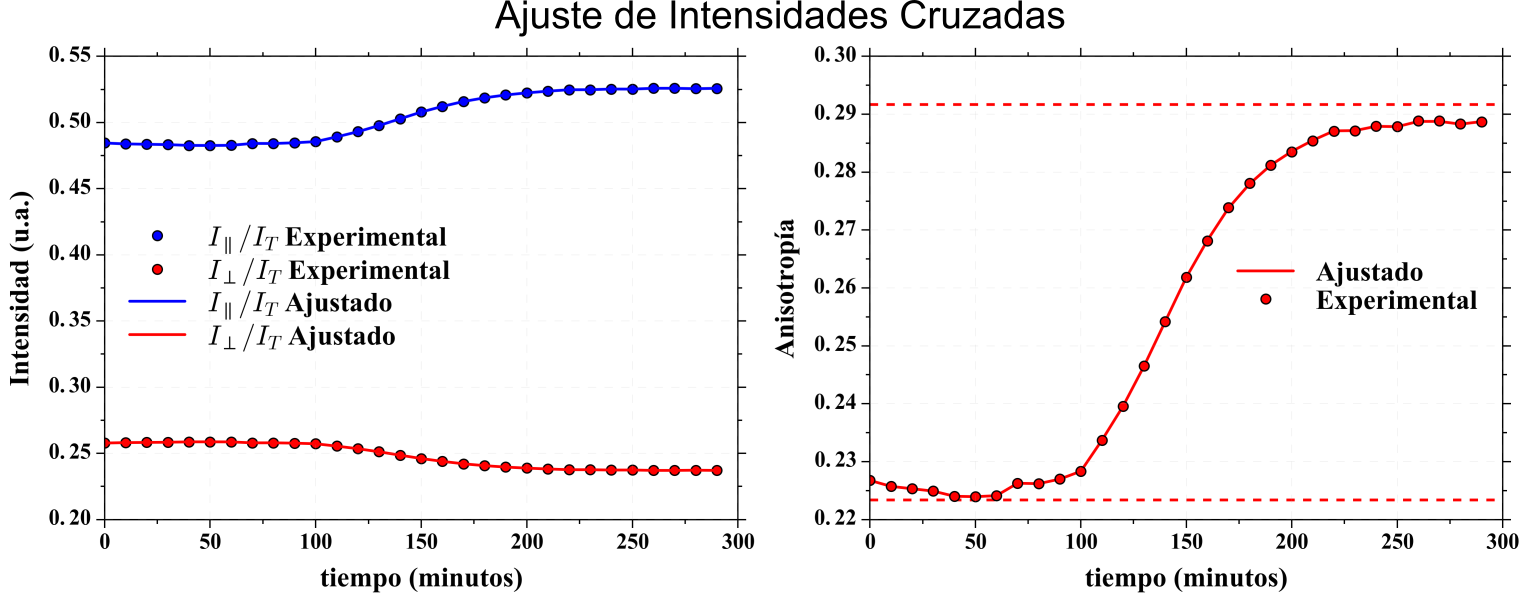
\includegraphics[width=0.9\textwidth]{./img/Cap4/Int_r_Fits.png}
    \caption{Ajustes realizados sobre las curvas intensidades cruzadas normalizadas. Puede apreciarse que hay la elevada similitud entre las curvas ajustadas y las intensidades, así como también entre la anisotropía obtenida a partir del ajuste y su contraparte experimental. Debe recalcarse que corresponde al ajuste de los mismos datos que la figura \ref{fig:Bad_Fits}}
    \label{fig:I_norm_Fit}
\end{figure}

\begin{figure}
    \centering
    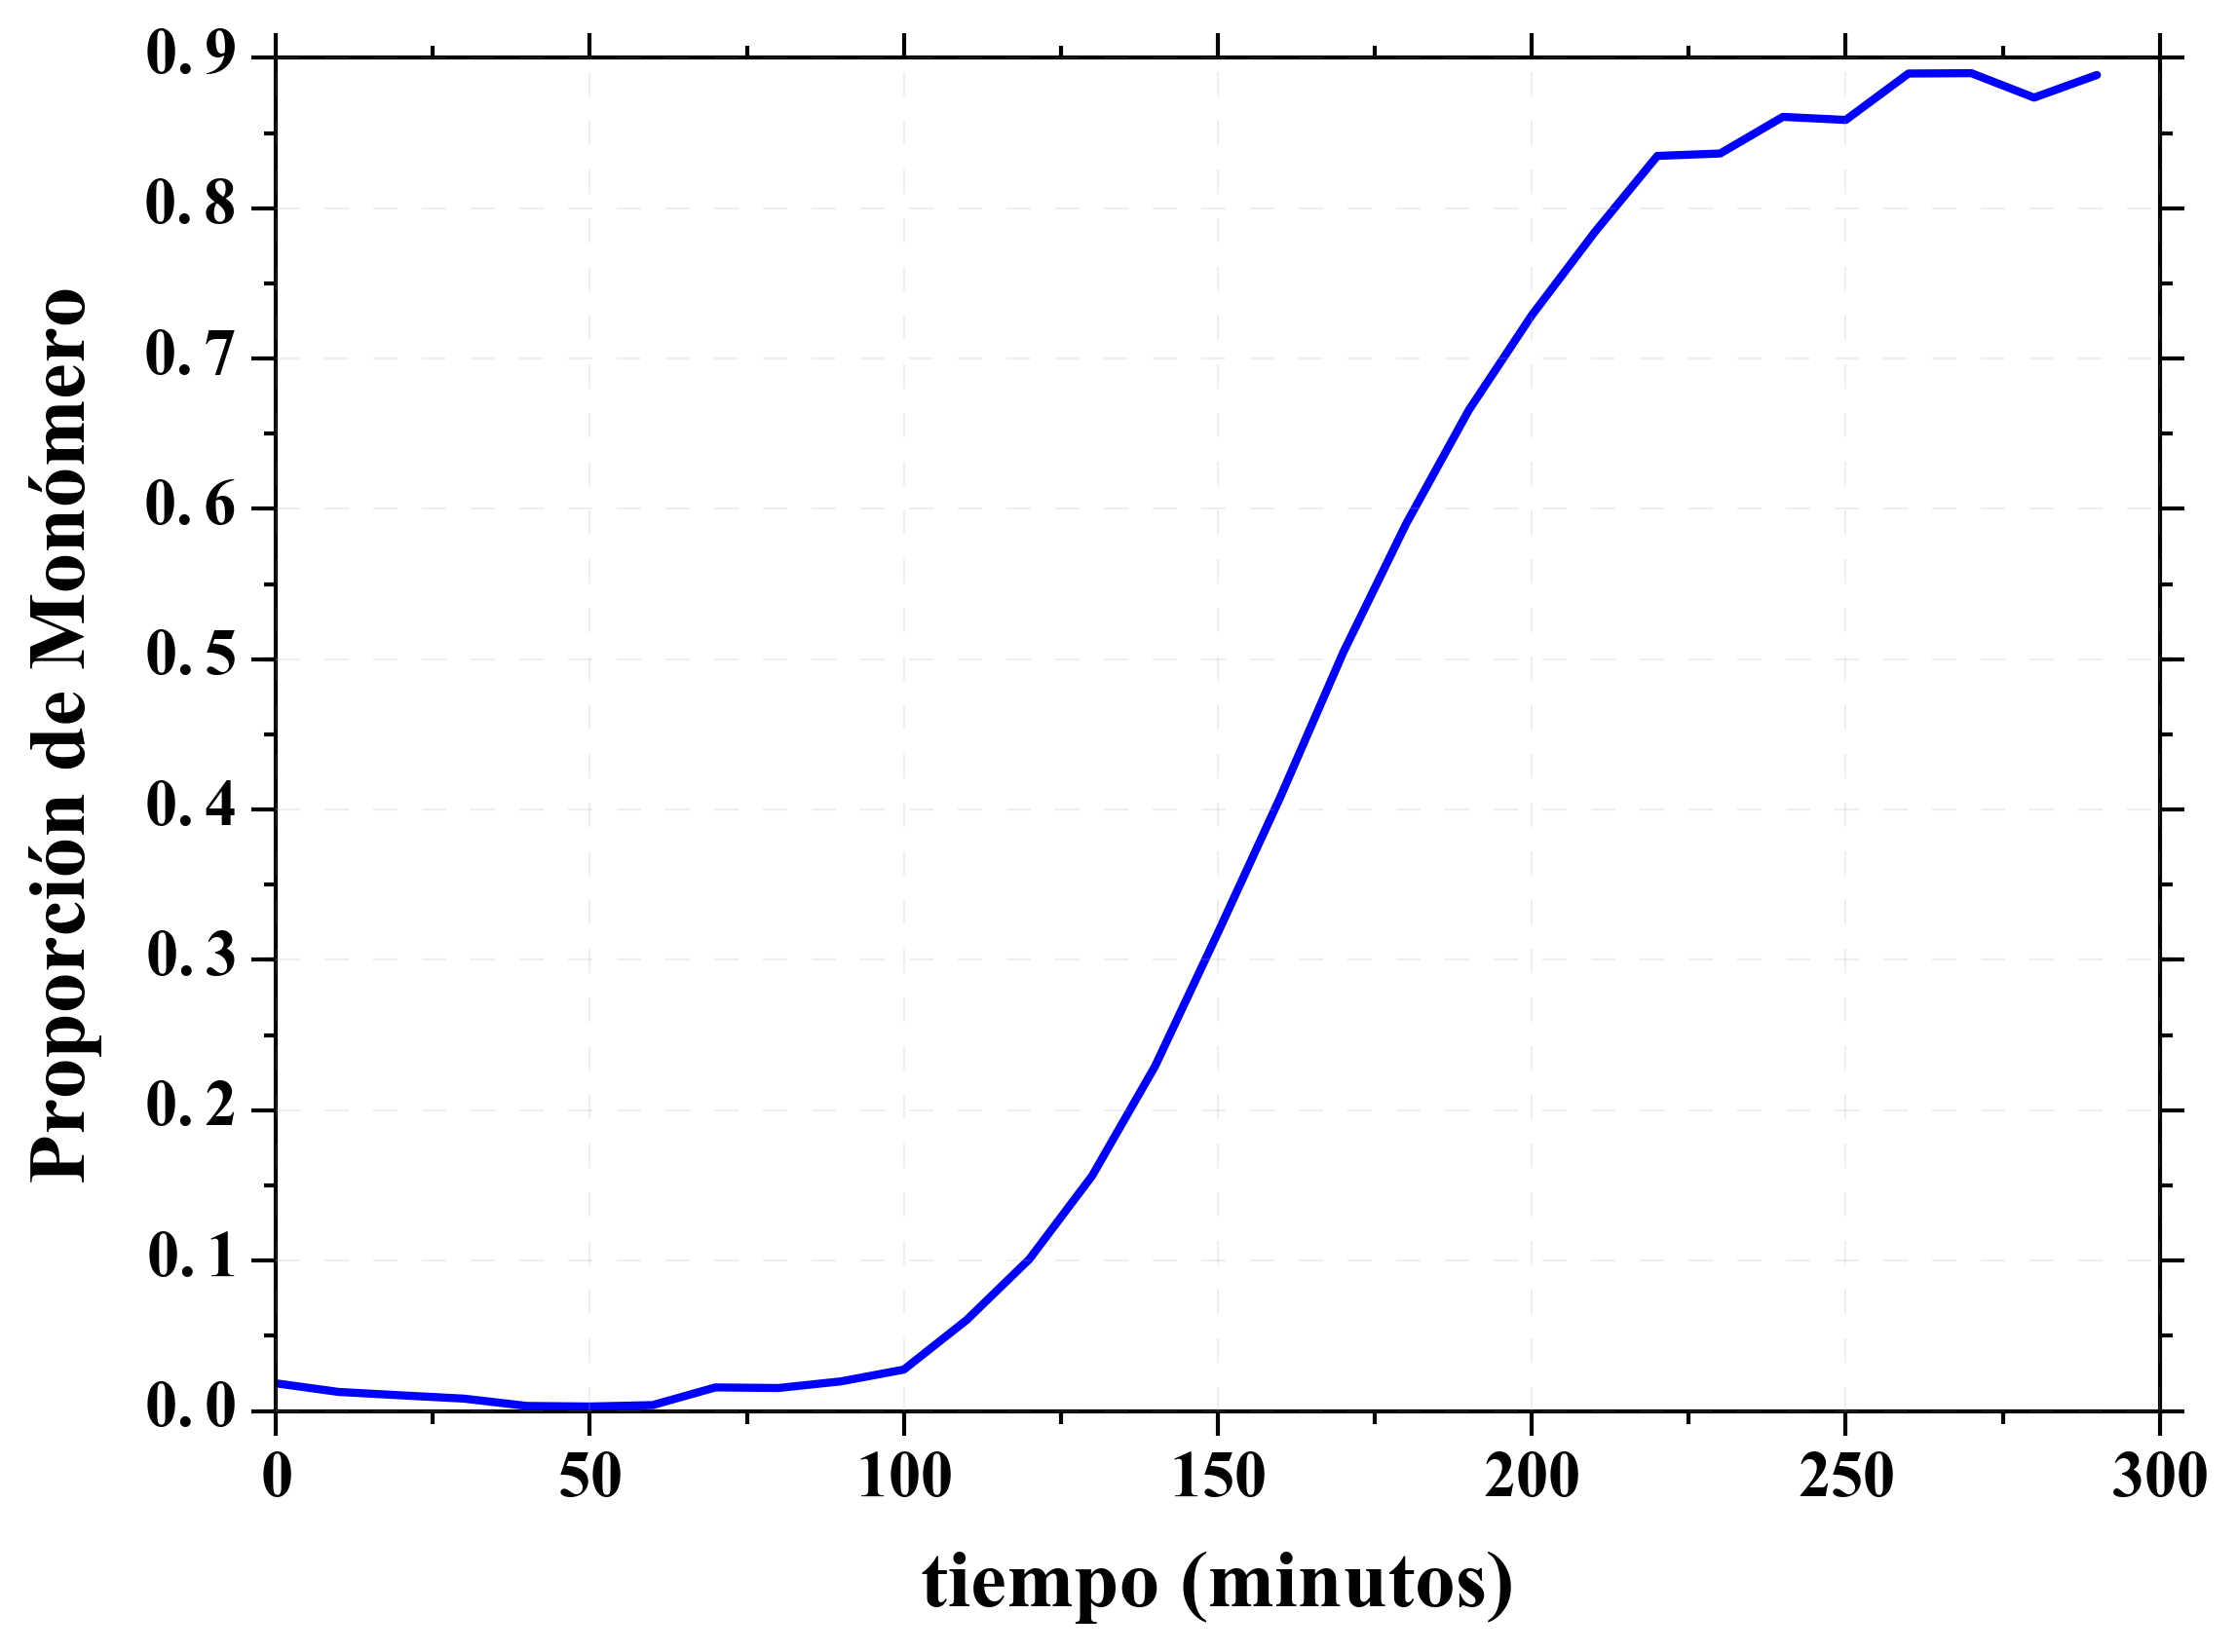
\includegraphics[width=0.6\textwidth]{./img/Cap4/Int_r_Fit_mYFP.png}
    \caption{Ajustes realizados sobre las curvas intensidades cruzadas normalizadas. Puede apreciarse que hay la elevada similitud entre las curvas ajustadas y las intensidades, así como también entre la anisotropía obtenida a partir del ajuste y su contraparte experimental.}
    \label{fig:m}
\end{figure}

%%%%%%%%%%%%%%%%%%
\section{Recuperación del Estado del Sistema Biológico}

Habiendo utilizado los hallazgos presentados en el capítulo \ref{cap:microscopia} para hallar las curvas de proporción de sensor en estado monomérico, se procedió a utilizar los métodos presentados en capítulo \ref{cap:modelo} para hallar el estado de la caspasa sensada. Luego, se procedió a calcular $\Delta m$ y $\Delta m/d$ como se mencionó previamente.

Con el objetivo de calcular $\Delta m$, se utilizó un filtro Savitzky-Golay para disminuir el ruido experimental y calcular la derivada temporal de $m$ utilizando más puntos que si utilizácemos un simple cálculo de cociente incremental. Aunque en muchos casos la curva obtenida no se condice con la teoría y aporta información del sistema, se pueden encontrar curvas como las presentadas en la figura \ref{fig:Deltams}. Esto genera problemas para estudiar diferencias en los tiempos de activación ya que muchas veces no podemos apreciar las curvas correspondientes a los tres sensores de una misma célula.

A continuación, se calcularon las curvas de $\Delta m/d$ para todas las curvas halladas. Desde el punto de vista numérico, este cálculo combina la problemática de calcular una derivada numérica con la necesidad de dividir por un factor que tiende a cero. Para evitar problemas al calcular divisiones por números chicos, se filtraron los valores de $d$ que eran considerados demasiado pequeños para el cálculo de $\Delta m/d$. De esta forma, se obtuvieron algunas curvas ideales, como la presentada en la figura \ref{fig:Deltams}, donde algunos puntos de la curva no pueden ser calculados, pero se puede apreciar gran parte del perfil de subida. El mayor inconveniente de estas curvas es que al no poseer información sobre los puntos más tardíos, cuando esta se normaliza, cambia la pendiente y no puede ser analizable.

\begin{figure}
    \centering
    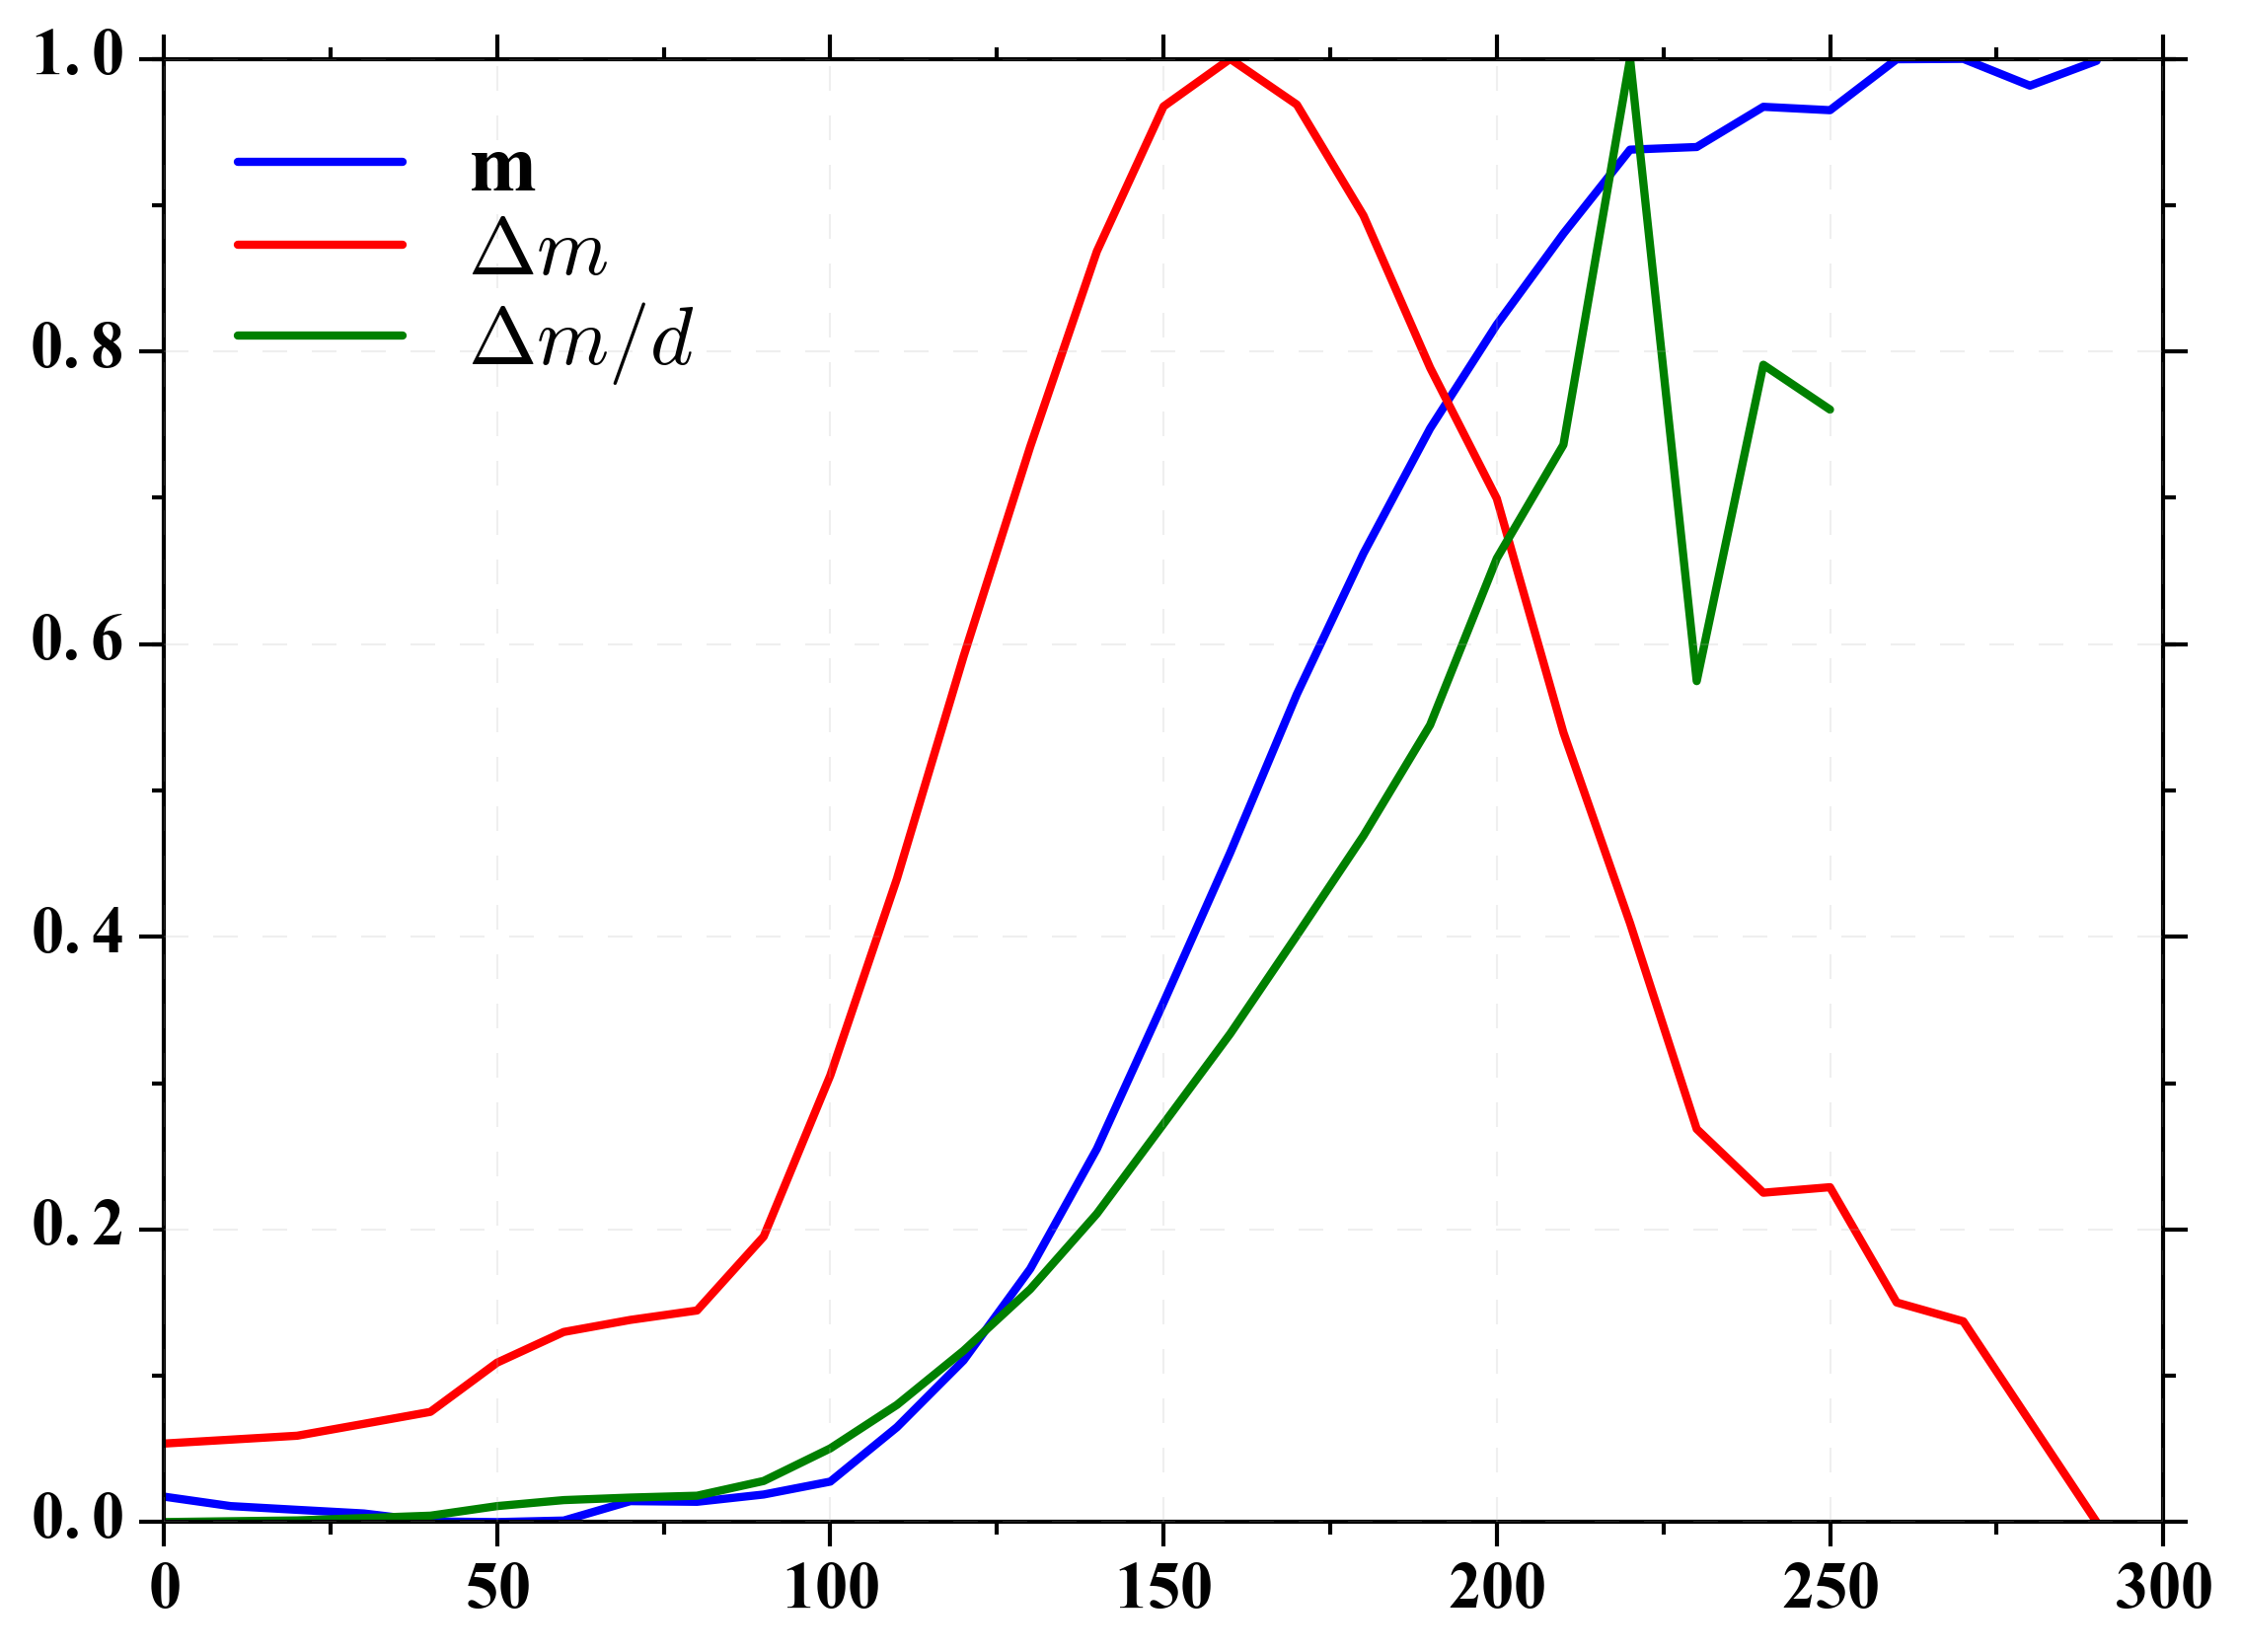
\includegraphics[width=0.6\textwidth]{./img/Cap4/Deltams.png}
    \caption{Gráfico de proporción de monómero en función del tiempo obtenido a partir de la transformación realizada. Se superponen los gráficos correspondientes a $\Delta m$ y $\Delta m/d$, que se corresponden a la caspasa en complejo con sensor y la proporción de caspasa activa en el momento.}
    \label{fig:m}
\end{figure}

Se planteó como corrección a futuro aumentar la resolución temporal para mejorar el cálculo de la derivada temporal. Debe considerarse que disminuir a la mitad el tiempo entre imágenes implica duplicar la cantidad de éstas, tornando más extenso el procesamiento de imágenes, u obligando a tomar imágenes de menos células. Por otro lado, los experimentos control que deben ser añadidos a la adquisición de imágenes permitirán determinar si el sensor comienza en estado dimérico en su totalidad, así como si culmina totalmente clivado. Esto puede ser utilizado para mejorar las aproximaciones sobre la curva de $d$ y así corregir aún más $\Delta m/d$.


%%%%%%%%%%%%%%%%%%%
\section{Ajuste Mediante Cinética Enzimática}

Con el objetivo de obtener una curva correspondiente a la proporción de caspasa activa, se diseño un método de ajuste de $m$ basado en cinética enzimática, presentado en la sección \ref{sec:CineticaEnzimatica}. Para ello, se truncó la cascada enzimática a nivel de la caspasa y solo se considero una fuente de caspasa tal que su proporción de caspasa activa, o enzima, poseía una forma funcional sigmoidea. Luego, los parámetros a ajustar correspondientes a la enzima son el tiempo en que la mitad de la enzima total aparece y la tasa de aparición de esta.

En este caso, la curva que se tiene disponible para ajustar es $m$, y los parámetros libres son los correspondientes a la aparición de enzima, así como todas las constantes de reacción. Debido a la gran cantidad de parámetros libres, resultaba fácil confeccionar ajustes que describan fielmente la forma de $m$, pero las curvas correspondientes a la caspasa que se obtenían eran extremadamente variables, y muchas veces carecían de sentido biológico.

Considerando que la cantidad de complejo sustrato:enzima es al menos cuatro ordenes de magnitud más chico que las cantidades de enzima, sustrato o producto (caspasa, dímeros o monómeros) y teniendo en cuenta que la velocidad de depleción de complejo es mucho mayor que la de sustrato, podemos aproximar la cinética enzimática de la siguiente forma

\begin{align}
    \frac{ds}{dt} =& - k_c se \label{eq:cin_sens}\\
    \frac{de}{dt} =& \nu(t)\\
    \frac{dp}{dt} =& 2 k_c se, \label{eq:cin_prod}\\
\end{align}

\noindent donde hay una única constante de reacción $k$ que combina todas las anteriores, y $\nu(t)$ corresponde a la fuente de enzima (caspasa) y es la derivada de la función sigmoidea, a saber,

\begin{equation}
    \nu(t) = A k \frac{e^{-k(t-t_0)}}{1 + e^{-k(t-t_0}},
\end{equation}

\noindent donde $A$ es la amplitud, tomada como 1 ya que corresponde a proporción de caspasa activa, $k$ es la tasa de aparición de caspasa, mientras que $t_0$ es el momento en que ya apareció la mitad de la caspasa activa.

Con el objetivo de validar este método de ajuste donde se varían los parámetros de la cinética enzimática hasta obtener la curva que mejor describe a $m$, se filtraron y analizaron datos correspondientes a un experimento control. Este consistió en diseñar los biosensores de forma tal que en una misma célula todos los biosensores sean clivados por la misma caspasa. De esta forma, se obtuvieron curvas de anisotropía para células que expresaban los tres sensores, pero su secuencia específica de clivaje es reconocida únicamente por la caspasa-3 u -8.

Si se tiene en cuenta que la caspasa tiene la misma constante de reacción para todos los sensores que tienen la secuencia específica reconocida por ella, se espera que los tres sensores se activen simultáneamente y tengan los mismos tiempos de activación. Podemos apreciar en la figura \ref{fig:OneCasp_Fit_m} las curvas de caspasa que se obtienen luego de ajustar las curvas de proporción de monómero. Al mismo tiempo, se presenta un gráfico del ajuste para tres pares de fluoróforos de la misma célula, mostrando la superposición entre estos.

\begin{figure}
    \centering
    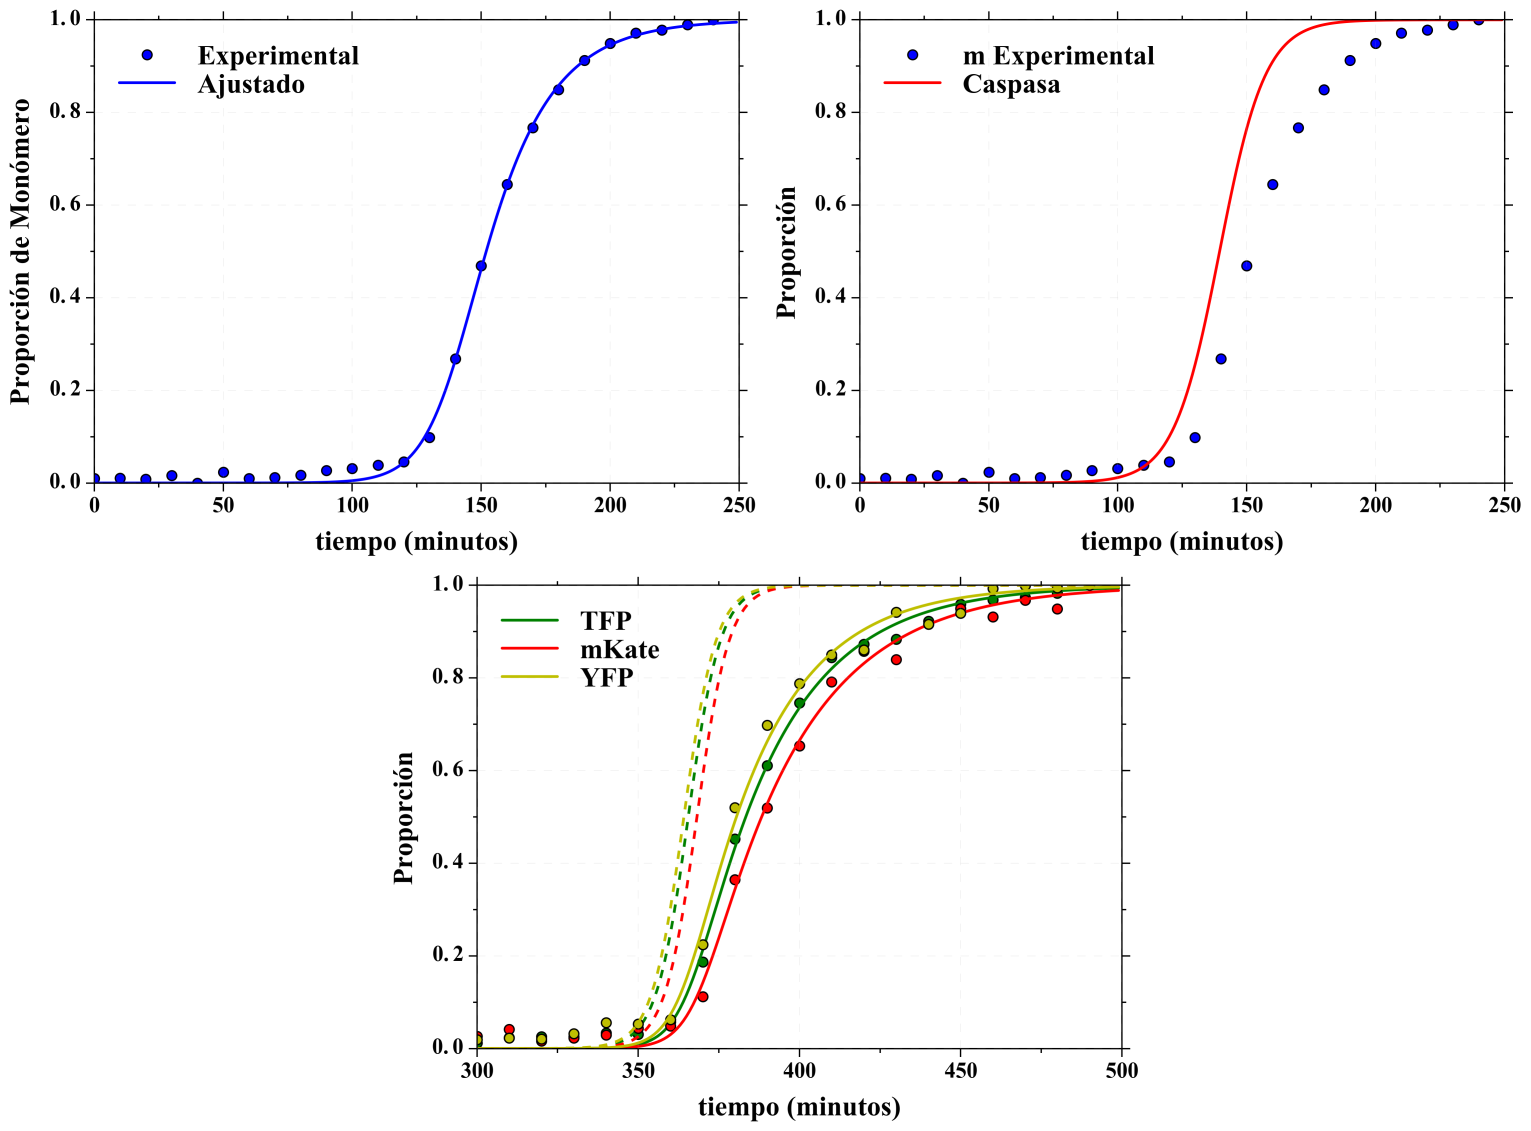
\includegraphics[width=0.9\textwidth]{./img/Cap4/OneCasp_Fit_m.png}
    \caption{Gráfico de los datos obtenidos de la proporción de sensor en estado monomérico. Se superponen el ajuste mediante cinética enzimática del cual se obtuvieron la proporción de monómero ajustada y la proporción de caspasa activa. En la sección inferior se presentan los ajustes realizados sobre tres caspasas de la misma célula, mostrando la validación del método con el caso control.}
    \label{fig:OneCasp_Fit_m}
\end{figure}

A continuación para validar este método, será necesario corroborar que los tiempos de activación, definidos como el tiempo que tarda la curva en llagar a cierto porcentaje de su valor máximo son los mismos para todas las caspasas. Luego, se consideraron los tiempos de activación al 10$\%$ y al 50$\%$ para cada par de fluoróforos y se graficaron uno contra otro. A partir de estos conjuntos de puntos, se calcularon las correspondientes regresiones lineales y se presentan sus gráficos en la figura \ref{fig:OneCasp_reg}. Los valores obtenidos para la regresión lineal correspondiente a usar el tiempo de activación de caspasa al 10$\%$ fueron para TFP contra YFP $-10.7 \pm 9.2$ de ordenada al origen y $1.02 \pm 0.03$ de pendiente; y para TFP contra mKate $-5.30 \pm 5.82$ de ordenada al origen y $1.01 \pm 0.02$ de pendiente. Por otro lado, utilizando la caspasa al 50$\%$ como tiempo de activación se aprecian para TFP contra YFP $-11.48 \pm 15.78$ de ordenada al origen y $1.03 \pm 0.05$ de pendiente, mientras que para TFP contra mKate se obtuvieron $2.45 \pm 9.95$ de ordenada al origen y $0.97 \pm 0.03$ de pendiente. En resumen, estos casos se superponen con la recta identidad que significa que este método es consistente al detectar la activación de la caspasa por igual para los tres sensores.

%p0 = -10.74 \pm 9.21
%p1 = 1.02 \pm 0.03


%p0 = -5.30 \pm 5.82
%p1 = 1.01 \pm 0.02


%p0 = -11.48 \pm 15.78
%p1 = 1.03 \pm 0.05


%p0 = 2.45 \pm 9.95
%p1 = 0.97 \pm 0.03

\begin{figure}
    \centering
    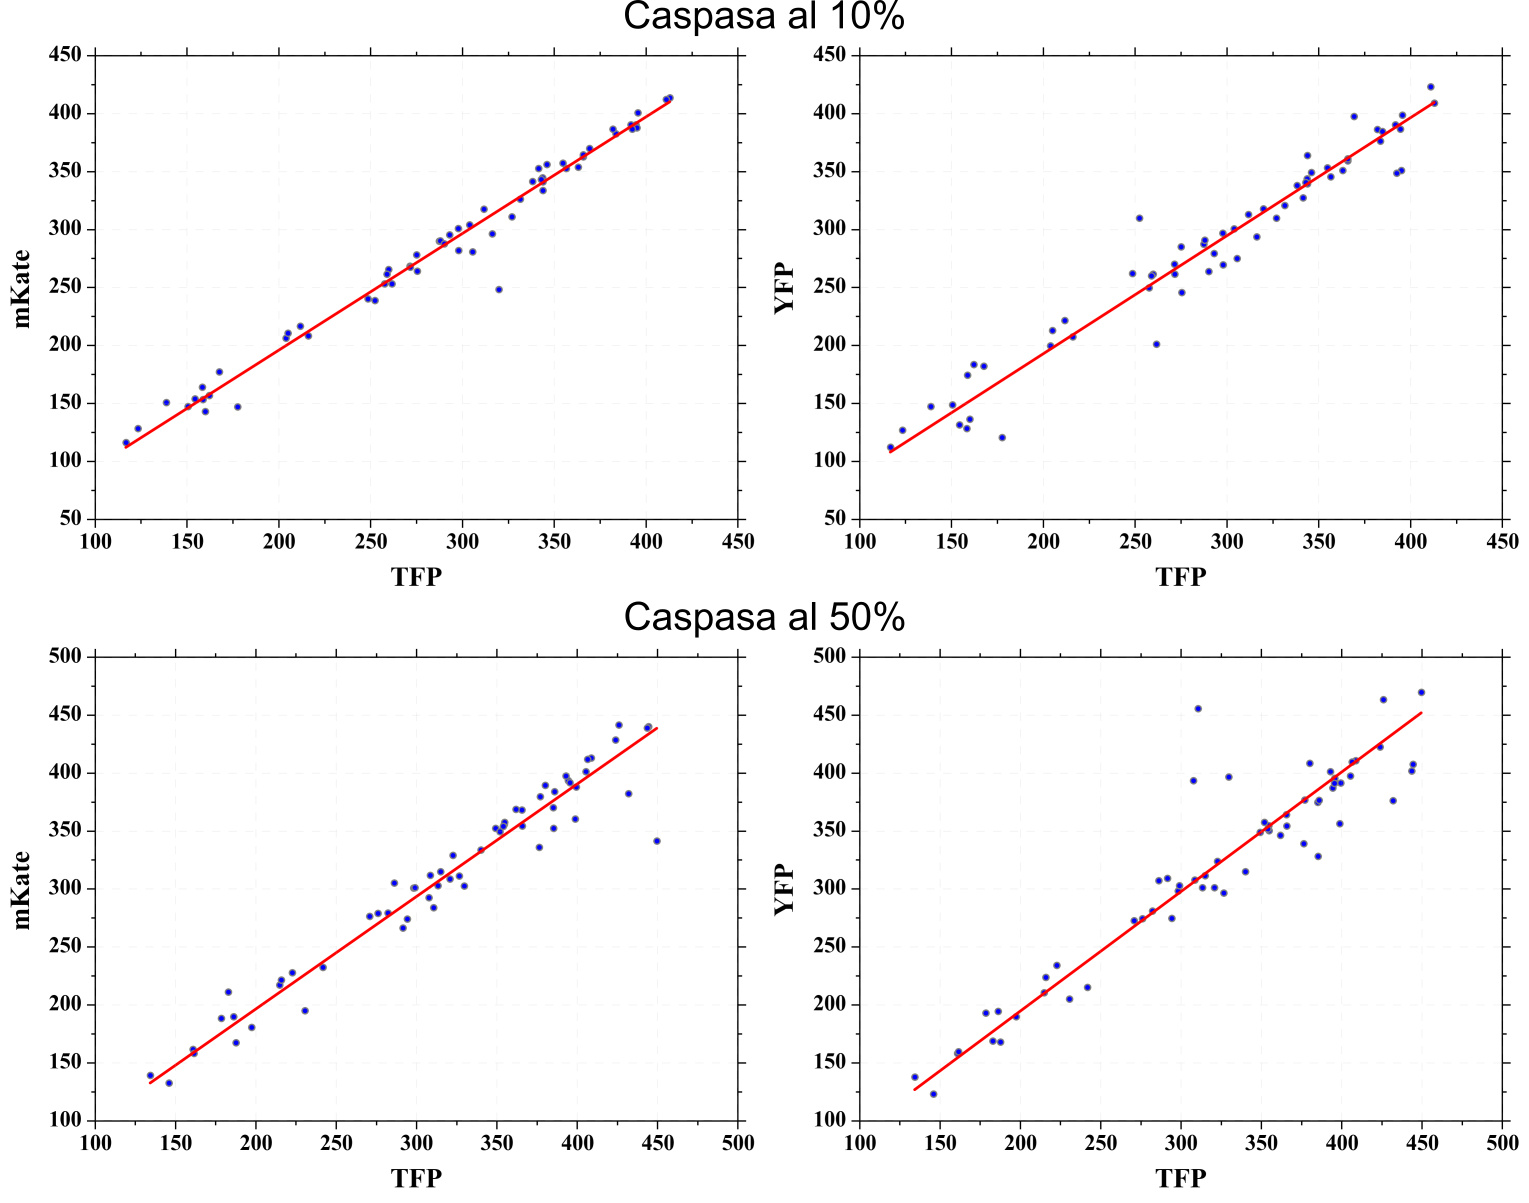
\includegraphics[width=0.9\textwidth]{./img/Cap4/CaspReg.png}
    \caption{Se graficaron los tiempos de activación obtenidos para 10$\%$ o 50$\%$ de activación de caspasa uno contra otro. La regresión lineal de estos datos permite constatar que efectivamente se trate del mismo parámetro ya que cada sensor medía la misma caspasa.}
    \label{fig:OneCasp_reg}
\end{figure}

%Por otro lado, es interesante comparar el método de tiempos de activación de caspasas con utilizar únicamente la anisotropía. Aunque ya mostramos que esto no es correcto ya que ignora varios fenómenos que dan lugar a variaciones en las curvas de anisotropía, . Entre estos, está el efecto que una relación entre brillos ($b$) distinto de 1 tiene sobre la pendiente de esta curva.

Por otro lado, podríamos retroceder y utilizar únicamente las curvas de anisotropía para encontrar en que momento asciende un 10$\%$ o 50$\%$ de su amplitud. Aunque se mostró en el capítulo \ref{cap:microscopia} que hacer esto implica ignorar efectos como, la variación de pendiente producida por una relación de brillos ($b$) distinta a 1, veamos si de todas formas es consistente y solo tiene un sesgo respecto del otro método. Para 10$\%$ de anisotropía se obtuvieron para TFP contra YFP $-21.26 \pm 8.95$ de ordenada al origen y $1.06 \pm 0.03$ de pendiente; para TFP contra mKate se obtuvo $-14.71 \pm 7.65$ de ordenada y $1.05 \pm 0.03$ de pendiente. Mientras que si utilizamos 50$\%$ de ascenso se obtienen para TFP contra YFP $-12.14 \pm 5.92$ de ordenada y $1.02 \pm 0.02$ de pendiente y para TFP contra mKate $-13.57 \pm 5.73$ de ordenada y $1.03 \pm 0.02$ de pendiente. Dado que en general hay una desviación respecto de la recta identidad, esto muestra que utilizar  los tiempos de activación obtenidos a partir de las caspasas es más robusto y consistente.

%p0 = -21.26 \pm 8.95
%p1 = 1.06 \pm 0.03


%p0 = -14.71 \pm 7.65
%p1 = 1.05 \pm 0.03


%p0 = -12.14 \pm 5.92
%p1 = 1.02 \pm 0.02


%p0 = -13.57 \pm 5.73
%p1 = 1.03 \pm 0.02

\begin{figure}
    \centering
    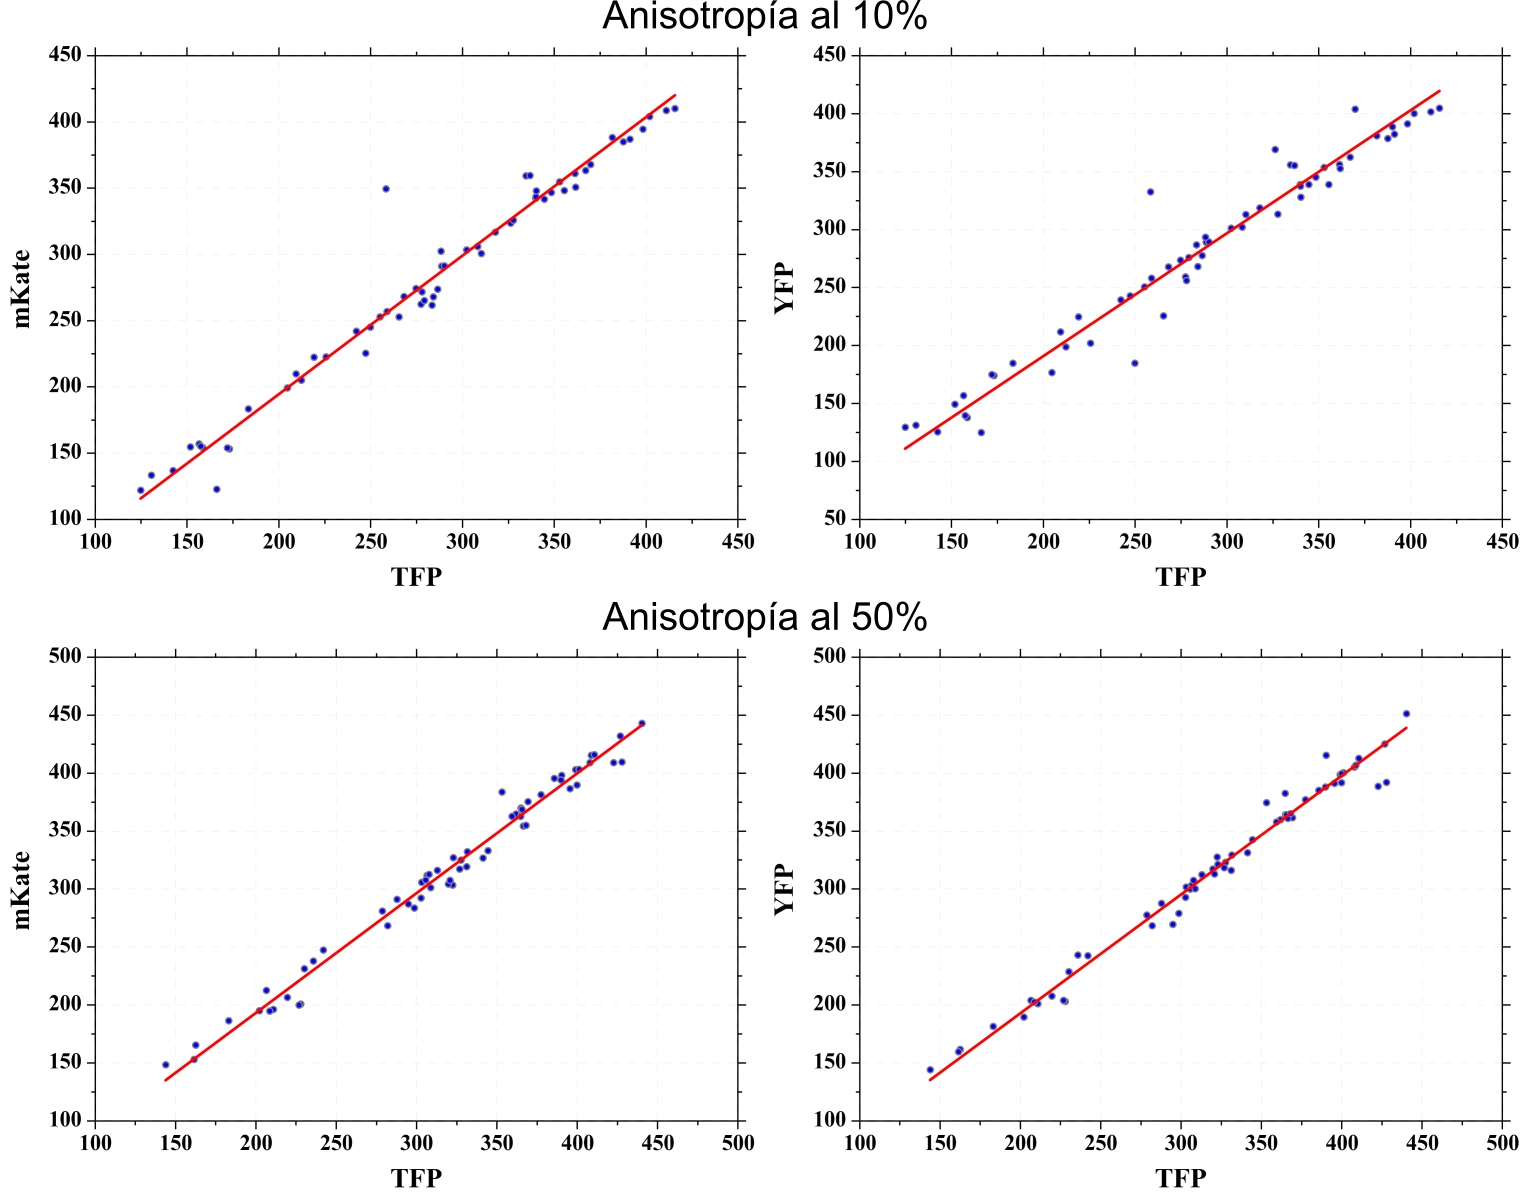
\includegraphics[width=0.9\textwidth]{./img/Cap4/AnisReg.png}
    \caption{Se graficaron los tiempos de activación obtenidos para 10$\%$ o 50$\%$ de activación de anisotropía uno contra otro. La regresión lineal de estos datos permite constatar que efectivamente se trate del mismo parámetro ya que cada sensor medía la misma caspasa.}
    \label{fig:OneCasp_reg_anis}
\end{figure}

%A partir de las regresiones lineales presentadas en las figuras \ref{fig:OneCasp_reg} y \ref{fig:OneCasp_areg}, podemos concluir que los ajustes mediante las simulaciones de cinética enzimática, no solo brindan información valiosa sobre el estado del sistema, sino que también son más robustas para comparar tiempos de iniciación.


%%%%%%%%%%%%%%%%%%%%%%
\section{Tiempo de Activación}

\subsection{Tiempos de Activación Observados}
Luego de validar el ajuste mediante las simulaciones de cinética enzimática, se procedió a aplicar el procedimiento a todas las curvas halladas experimentalmente. De este análisis fue posible obtener los tiempos de activación definidos previamente para las caspasas-3, -8 y -9 en una misma célula. Como se detalla en el trabajo de \textit{Sorger et al.}\cite{Sorger2008}, el tiempo en que se inicia la cascada apoptótica es muy variable intercelularmente, pero el orden y la diferencia entre los tiempos de activación de cada caspasa se mantiene relativamente constante entre las distintas células. Por esta razón, en lugar de analizar estadísticamente los tiempos de activación de las distintas caspasas, se estudiaron las diferencias entre los tiempos de activación.

\begin{figure}
    \centering
    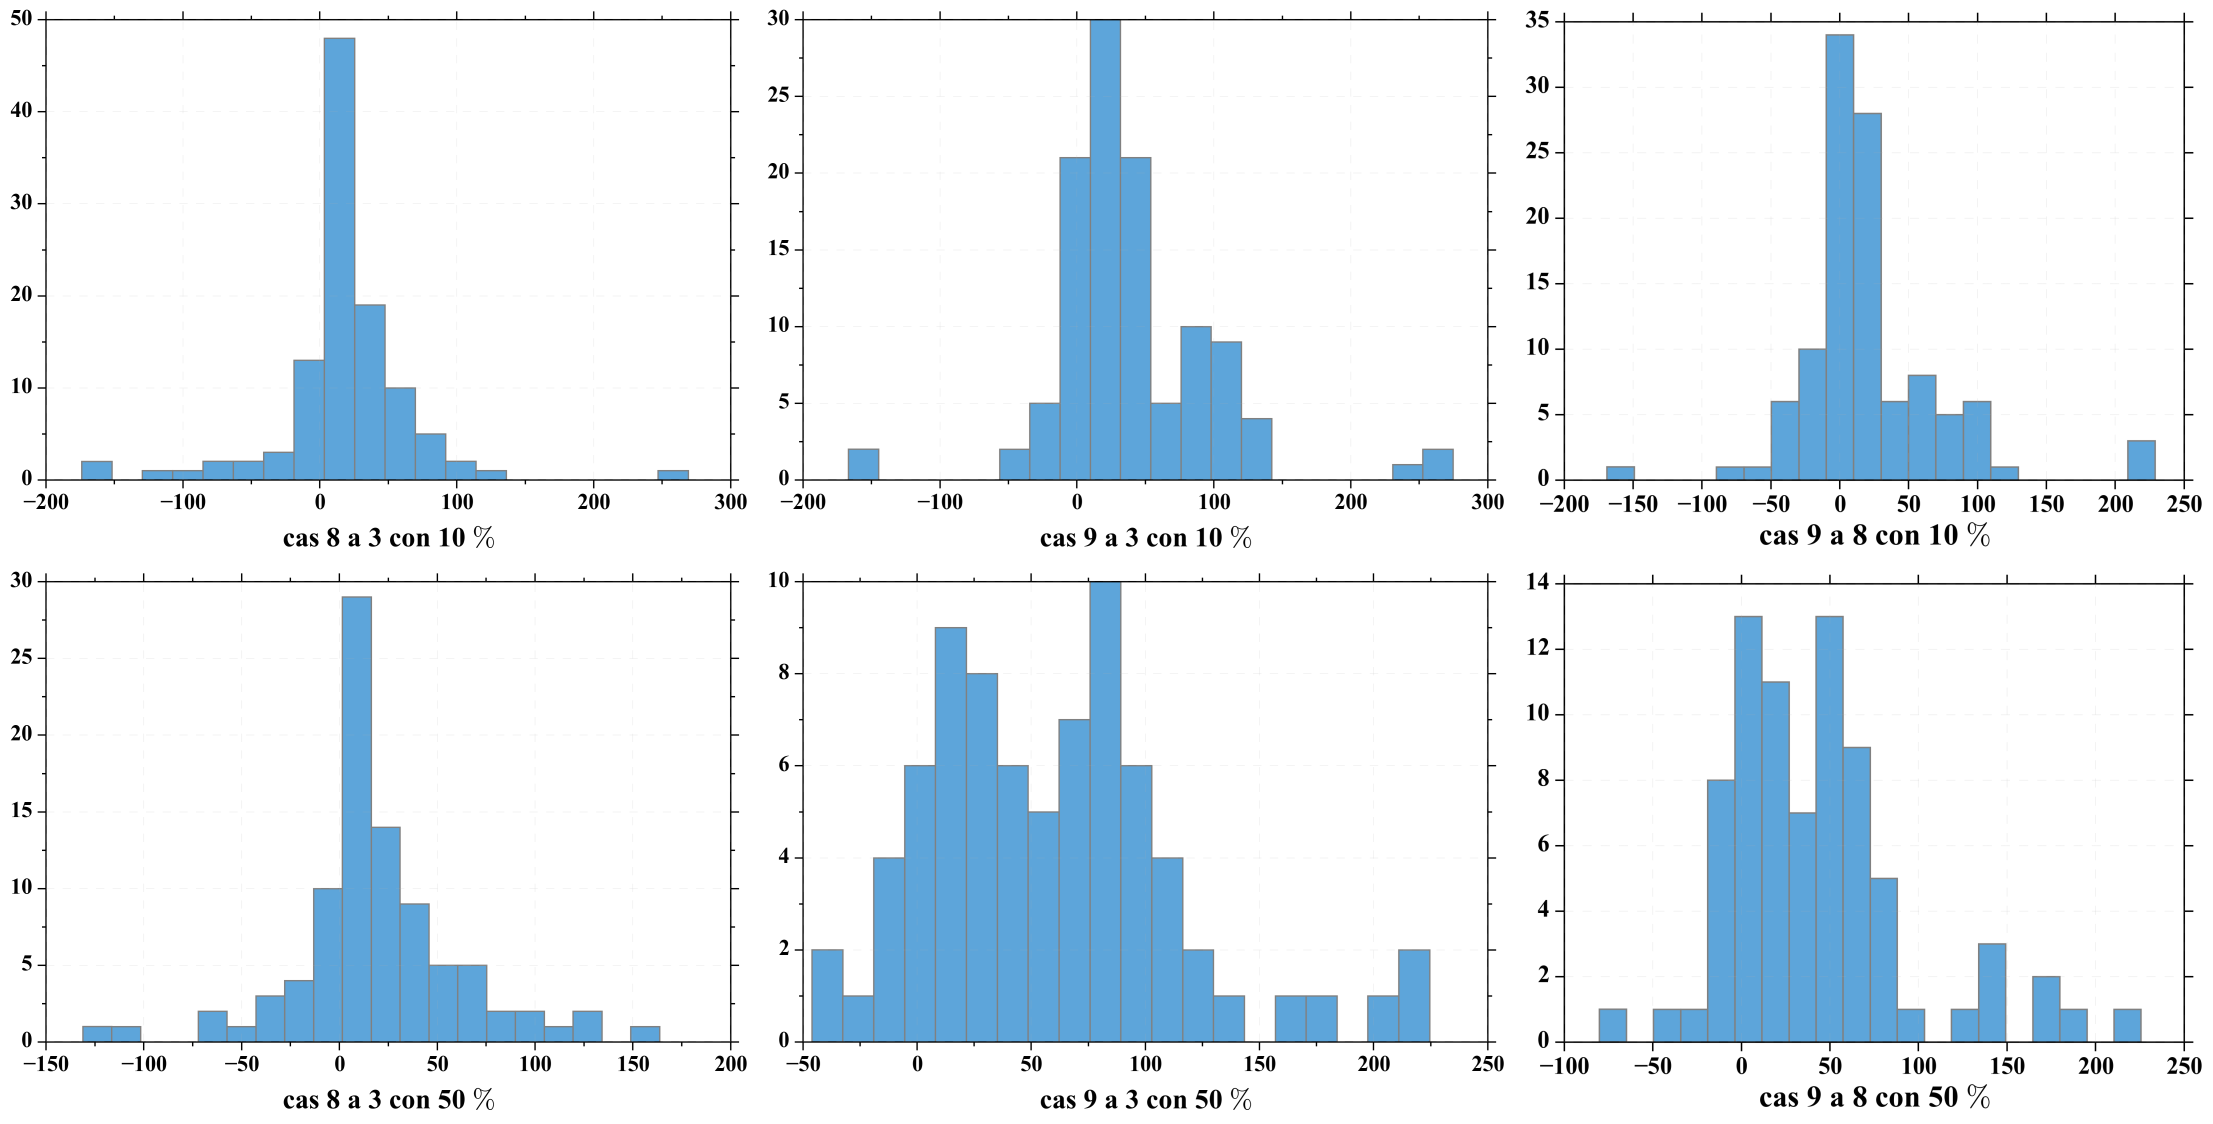
\includegraphics[width=0.9\textwidth]{./img/Cap4/HistTimes.png}
    \caption{Se presentan histogramas de las diferencias entre los tiempos de activación de cada caspasa. }
    \label{fig:OneCasp_reg_anis}
\end{figure}

Al analizar los tiempos de activación al 10$\%$ se apreció que hay una diferencia temporal de $17.4\pm4.8$ desde la caspasa-8 a la -3, $21.8\pm5.0$ desde la -9 a la -8 y, por último, $40.6\pm5.6$ desde la caspasa-9 a la -3. Por otro lado, si consideramos el tiempo de activación como el momento en que el 50$\%$ de la caspasa se haya activa se obtuvieron diferencias de tiempo desde la caspasa-8 a la -3 de $18.8\pm4.5$, desde la caspasa-9 a la -8 de $42.2\pm6.0$ y de la caspasa-9 a -3 de $57.9\pm6.4$. De estos resultados puede deducirse que la caspasa-3 es la primera en iniciarse, seguida de cerca por la caspasa-8, y un tiempo después la caspasa-9. Se debe destacar que si prestamos especial atención a ambos estimadores, apreciamos que la caspasa-8 comienza temprano con la caspasa-3, pero luego se retrasa y alcanza su 50$\%$ de activación unos minutos antes que la caspasa-9.


\subsection{Tiempos de Activación Estimados}

A partir del modelo matemático adapatado en el capítulo \ref{cap:modelo}, podemos estimar la separación temporal entre las activaciones del 10$\%$ o 50$\%$ de caspasas. En primer lugar, cabe destacar que aunque parezca incoherente con el esquema de la red, la primer caspasa en llegar a una activación del 10$\%$ es la caspasa-3, seguida de cerca temporalmente por la caspasa-8. Un tiempo más prolongado, comparado con la separación entre las caspasas-3 y -8, separa a la activación del 10$\%$ de la caspasa-9. Experimentalmente podemos apreciar que el orden se conserva, aunque la separación entre las activaciones observadas experimentalmente son equiespaciadas.

Por otro lado, si analizamos las separaciones temporales entre las activaciones del 50$\%$ de caspasa, podemos apreciar que se invierten los ordenes de activación entre las caspasas-8 y -9, siendo la caspasa-3 la primera en activarse.En este caso, apreciamos en el experimento que la caspasa-8 sufre un retraso o la caspasa-9 se adelanta, como se explico previamente, pero este efecto no es suficiente para obtener una inversión en el orden de activación de las caspasas.


%%%%%%%%%%%%%%%%%%%%%%
\section{Orden de Activación Según Estímulo}

Hasta ahora, se consideró como estímulo un ligando que actúa a nivel de los receptores de muerte, como TNF-$\alpha$. El estímulo utilizado en los experimentos realizados fue la staurosporina. Aunque no hay certeza sobre la vía estimulada por la misma, los datos experimentales presentados y analizados sugieren que se trata de una estimulación de la vía extrínseca.

Con el objetivo de contrastar el orden de activación de las caspasas según que vía se ve estimulada, se generó una variante del modelo matemático que no contiene ligando para actuar a nivel del receptor. Por otro lado, en esta variante, parte de la proteína Bax comienza activa para inicializar la vía intrínseca. Bax esta involucrada en la respuesta celular a daño interno por especies reactivas del oxígeno.

\begin{figure}
    \centering
    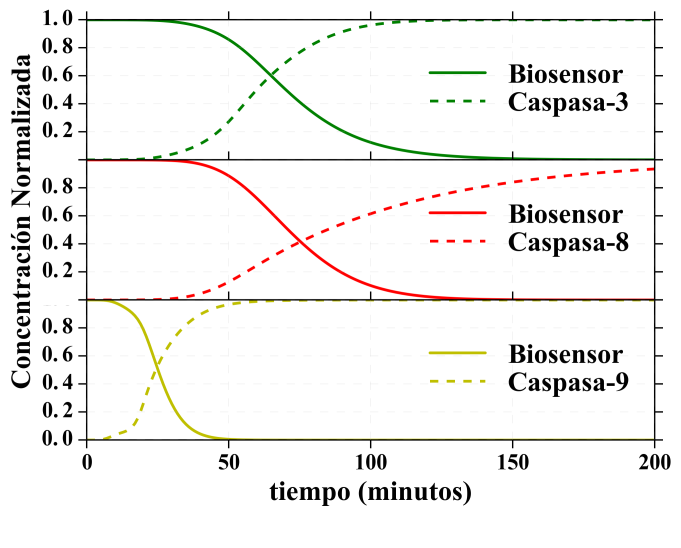
\includegraphics[width=0.8\textwidth]{./img/Cap4/IntAct.png}
    \caption{Gráficos de proporción de caspasa activa y sensor sin clivar en función del tiempo para las tres caspasas de interés. En esta simulación se estimuló la vía intrínseca en lugar de la extrínseca y puede apreciarse una alteración en el orden en que se activan las caspasas.}
    \label{fig:IntAct}
\end{figure}

En esta variante de iniciación de vía intrínseca, se aprecia que la caspasa-9 alcanza primero el 10$\%$, así como también el 50$\%$ de activación primera. Un tiempo después la sigue la caspasa-3, mientras que la caspasa-8 es la última en llegar a los porcentajes de activación seleccionados. Estas diferencias en los ordenes de activación nos permiten determinar cual es la vía de entrada en apoptosis tomada por la célula.